% !TeX program = xelatex
% XeLaTeX academic report template (Ferrari case study)

\documentclass[12pt,a4paper]{report}

% ---------- XeLaTeX font and language ----------
\usepackage{fontspec}
\usepackage{polyglossia}
\setdefaultlanguage{english}
\defaultfontfeatures{Ligatures=TeX,Scale=MatchLowercase}
% Body: readable, print-friendly serif. Headings: clean motorsport-style sans.
\setmainfont{TeX Gyre Pagella}
\setsansfont{TeX Gyre Heros}
% Monospace font: TeX-shipped, avoids OS font dependency.
\setmonofont{Latin Modern Mono}
\newfontfamily\HeadingFont{TeX Gyre Heros}

% ---------- Page layout and spacing ----------
\usepackage[a4paper,margin=1in]{geometry}
\usepackage{setspace}
\onehalfspacing
\setlength{\parskip}{0.6em}
\setlength{\parindent}{0pt}

% --- REQUIRED PACKAGES(sharaf) ---
\usepackage{longtable} % <--- ADD THIS for the multi-page table
\usepackage{fontspec}      % Standard for XeLaTeX
\usepackage{booktabs}      % Professional tables
\usepackage{tabularx}      % Auto-width columns
\usepackage{array}         % Custom column definitions
\usepackage{caption}       % Better caption formatting
\usepackage{enumitem}      % For compact lists inside tables
\usepackage{tikz}          % For the diagram
\usetikzlibrary{arrows.meta, positioning, shadows, calc, decorations.pathreplacing}

% ---------- Visual identity (Ferrari-inspired, restrained) ----------
\usepackage{xcolor}
\definecolor{Charcoal}{RGB}{28,28,28}
\definecolor{MetalGray}{RGB}{120,120,120}
\definecolor{Ivory}{RGB}{250,248,242}
\definecolor{FerrariRed}{RGB}{200,16,46}
\color{Charcoal}

%----------- listings (for code snippets, if needed) ----------
\usepackage{listings}
\usepackage{xcolor}
\usepackage{graphicx}

\lstset{
    language=Matlab,
    basicstyle=\ttfamily\small,
    keywordstyle=\color{blue},
    commentstyle=\color{gray},
    stringstyle=\color{red},
    numbers=left,
    numberstyle=\tiny,
    frame=single,
    breaklines=true,
    captionpos=b
}

% ---------- Figures, tables, and floats ----------
\usepackage{graphicx}
\usepackage{booktabs}
\usepackage{longtable}
\usepackage{tabularx}
\usepackage{array}
\usepackage{caption}
\usepackage{float}
\usepackage{microtype}

% ---------- Section styling (technical, minimal) ----------
\usepackage{titlesec}


  \titleformat{\chapter}[display]
  {\HeadingFont\bfseries\Large\color{Charcoal}}
  {\HeadingFont\bfseries\color{MetalGray}\MakeUppercase{\chaptertitlename}\ \thechapter}
  {0.6em}
  {\MakeUppercase}
  [\vspace{0.4em}\color{FerrariRed}\rule{0.18\textwidth}{0.6pt}]

  \titleformat{\section}
  {\HeadingFont\bfseries\large\color{Charcoal}}
  {\thesection}
  {0.8em}
  {}
  [\vspace{0.25em}\color{FerrariRed}\rule{0.12\textwidth}{0.5pt}]

  \titleformat{\subsection}
  {\HeadingFont\bfseries\normalsize\color{Charcoal}}
  {\thesubsection}
  {0.8em}
  {}

  \titlespacing*{\chapter}{0pt}{-0.2cm}{0.8cm}
  \titlespacing*{\section}{0pt}{0.8cm}{0.3cm}
  \titlespacing*{\subsection}{0pt}{0.6cm}{0.2cm}

% ---------- Math and symbols ----------
\usepackage{amsmath,amssymb}

% ---------- Lists and links ----------
\usepackage{enumitem}
\usepackage[hidelinks]{hyperref}

% ---------- Headers & footers (technical briefing style) ----------
\usepackage{fancyhdr}
\pagestyle{fancy}
\fancyhf{}
\renewcommand{\headrulewidth}{0pt}
\renewcommand{\footrulewidth}{0pt}
\fancyhead[L]{\HeadingFont\small\color{MetalGray}\nouppercase{\rightmark}}
\fancyfoot[C]{\color{FerrariRed}\rule{0.65\textwidth}{0.5pt}\\[0.35em]{\HeadingFont\small\color{Charcoal}\thepage}}

\setlength{\headheight}{14.5pt}

% Ensure \rightmark shows section titles
\renewcommand{\chaptermark}[1]{\markboth{#1}{}}
\renewcommand{\sectionmark}[1]{\markright{#1}}

% ---------- Captions (muted red accent, minimal) ----------
\DeclareCaptionLabelFormat{ferrariaccent}{\textcolor{FerrariRed}{#1\ #2}}
\captionsetup{
  font=small,
  labelfont=bf,
  labelsep=quad,
  labelformat=ferrariaccent,
  textfont=it
}

% ---------- Figure/table placeholder box (no embedded images) ----------
\newcommand{\FerrariPlaceholder}[1]{%
  \begin{center}
    \setlength{\fboxsep}{10pt}%
    \setlength{\fboxrule}{0.4pt}%
    \fcolorbox{Charcoal}{Ivory}{\parbox{0.92\textwidth}{\centering\vspace{1.0cm}#1\vspace{1.0cm}}}
  \end{center}
}

% ---------- Bibliography ----------
\usepackage[backend=biber,style=authoryear,maxcitenames=2,maxbibnames=99]{biblatex}
\addbibresource{references.bib}

% ---------- Front matter helpers ----------
\usepackage{titling}
\usepackage{tocloft}

% ---------- Document metadata ----------
\newcommand{\ReportTitle}{Economics and Marketing Analysis of Ferrari}
\newcommand{\ReportSubtitle}{A Technical Economics and Marketing Report}
\newcommand{\ReportAuthor}{[Your Name]}
\newcommand{\ReportAffiliation}{[University Name]}
\newcommand{\ReportCourse}{[Course Name]}
\newcommand{\ReportInstructor}{[Instructor Name]}
\newcommand{\ReportDate}{December 2025}

\begin{document}

% ============================================================
% Cover page (minimalist technical layout)
% ============================================================
\begin{titlepage}
  	\thispagestyle{empty}
\vspace*{2.2cm}

{\HeadingFont\bfseries\fontsize{26}{30}\selectfont\color{Charcoal}\ReportTitle\par}
\vspace{0.35cm}
{\HeadingFont\fontsize{12}{16}\selectfont\color{MetalGray}\ReportSubtitle\par}

\vspace{0.9cm}
\color{FerrariRed}\rule{0.65\textwidth}{0.8pt}

\vspace{1.2cm}
{\HeadingFont\small\color{Charcoal}
\begin{tabular}{@{}ll@{}}
  	\textbf{Author} & \ReportAuthor\\
  	\textbf{Affiliation} & \ReportAffiliation\\
  	\textbf{Course} & \ReportCourse\\
  	\textbf{Instructor} & \ReportInstructor\\
  	\textbf{Date} & \ReportDate\\
\end{tabular}}

\vfill
{\HeadingFont\footnotesize\color{MetalGray}
Prepared as a technical academic report.}
\end{titlepage}

% ============================================================
% Declaration (separate page for clean cover)
% ============================================================
\chapter*{Declaration}
  	\thispagestyle{plain}
I declare that this report is my own work and that all sources used have been properly acknowledged.\par
\vspace{1.2cm}
Signature: \rule{7cm}{0.4pt}\par

% ============================================================
% Abstract
% ============================================================
\pagenumbering{roman}
\chapter*{Abstract}
This report presents an integrated economics and marketing analysis of Ferrari, focusing on how a luxury performance brand creates and captures value under conditions of scarcity, high willingness-to-pay, and intense reputational scrutiny. The study synthesizes core microeconomic concepts---demand, elasticity, cost structures, market power, pricing, and competitive interaction---with marketing frameworks such as STP, the marketing mix, brand equity, customer journey design, and digital marketing strategy \parencite{kotlerkeller2016,porter1980,varian2014}. The report evaluates Ferrari's product and service portfolio, distribution and communications model, pricing logic, and the firm's interaction with macroeconomic, technological, and regulatory environments. A qualitative SWOT and risk-opportunity assessment is provided, followed by strategic recommendations emphasizing sustainable growth, controlled exclusivity, digitally enabled relationship marketing, and long-term competitive resilience.

% ============================================================
% Acknowledgements (optional)
% ============================================================
\chapter*{Acknowledgements}
[Write short acknowledgements here, if required by your institution.]

% ============================================================
% Table of contents
% ============================================================
\tableofcontents
\listoftables
\listoffigures

\cleardoublepage
\pagenumbering{arabic}

% ============================================================
% Chapter 1
% ============================================================
\chapter{Introduction and Objectives of the Study}
\section{Background and Motivation}
Ferrari is widely recognized as a global symbol of performance engineering, racing heritage, and luxury brand exclusivity. Unlike mass-market automotive firms that compete primarily on volume, scale efficiencies, and broad-based segmentation, Ferrari competes in a market where constrained supply, brand mythology, product craftsmanship, and customer experience are central to value creation. This positioning makes Ferrari a relevant case for an integrated analysis that combines economics and marketing: the firm operates in a segment where demand is shaped by identity signaling, emotional utility, and social prestige, while costs reflect advanced engineering and a strong emphasis on quality, compliance, and design differentiation.

From an economic perspective, luxury durable goods provide a rich setting to analyze: price elasticity and income elasticity; intertemporal consumption; scarcity and rationing mechanisms; product differentiation and monopolistic competition; and strategic interaction with rivals. From a marketing perspective, Ferrari illustrates how brand equity is built and defended through controlled distribution, selective communications, experience design, and community management.

\section{Research Objectives}
The primary objectives of this study are:
\begin{enumerate}[label=\textbf{O\arabic*:},leftmargin=*]
  \item To summarize the core economics and marketing concepts relevant to analyzing a luxury automotive firm.
  \item To apply these concepts to Ferrari, describing the company context, organizational structure, and strategic approach.
  \item To evaluate Ferrari's marketing management, digital presence, and promotional methods.
  \item To analyze Ferrari's pricing strategy, value proposition, and segmentation-targeting-positioning (STP).
  \item To assess Ferrari's competitive environment and the economic logic of its business model.
  \item To produce a SWOT analysis and develop forward-looking recommendations.
\end{enumerate}

\section{Scope, Methodology, and Limitations}
\subsection{Scope}
The report focuses on Ferrari as a global organization, emphasizing marketing strategy and economic principles that can be analyzed using publicly observable information such as corporate communications, product portfolio characteristics, and typical industry conditions. The study considers both physical goods (vehicles and branded products) and related services (ownership services, aftersales, brand experiences, and digital services).

\subsection{Methodology}
The approach is qualitative and conceptual, combining:
\begin{itemize}[leftmargin=*]
  \item Literature-based frameworks in marketing and economics \parencite{kotlerkeller2016,varian2014}.
  \item Case study reasoning (mapping frameworks to Ferrari's observable strategy and brand behaviors).
  \item Structured strategic analysis tools (STP, 4Ps/7Ps, PESTEL, Porter five forces, and SWOT) \parencite{porter1980,porter1985}.
\end{itemize}

\subsection{Limitations}
This report does not rely on proprietary internal data. Quantitative claims (e.g., exact financials, production volumes, conversion rates) are avoided unless sourced from official disclosures. Where numerical analysis would typically be expected, the report provides structured placeholders for future insertion (tables/charts) and explains the logic and the type of data required.

% Placeholder
\begin{figure}[H]
  \centering
  \includegraphics[width=0.8\textwidth]{../team/1.1.jpg}
%\FerrariPlaceholder{[Figure 1: Research Framework Linking Economics and Marketing Concepts to Ferrari]}
\caption{Conceptual framework of the study (placeholder).}
\end{figure}

% ============================================================
% Chapter 2
% ============================================================
\chapter{Overview of Key Economics and Marketing Concepts}
\section{Foundational Economic Concepts}
\subsection{Demand, Utility, and Consumer Choice}
In microeconomics, consumer choice is typically modeled as the selection of a bundle of goods that maximizes utility subject to a budget constraint \parencite{varian2014}. Luxury consumption complicates this framework by introducing strong roles for symbolic utility (status signaling), social comparison, and identity expression. For Ferrari, the value to customers may derive from performance and craftsmanship (functional utility), but also from belonging, prestige, and heritage (symbolic utility). These aspects can shift demand curves outward even when functional substitutes exist.

\subsection{Elasticity}
Price elasticity of demand measures responsiveness of quantity demanded to changes in price. Luxury brands often seek to reduce price elasticity through differentiation and brand equity, making demand less sensitive to price within the relevant segment. Income elasticity is also particularly important: Ferrari demand may be correlated with high-income segments and wealth effects, implying sensitivity to macroeconomic cycles that affect high-net-worth consumers.

\subsection{Costs, Scale, and Learning}
Cost structure matters for pricing and strategic choices. Automotive manufacturing can exhibit large fixed costs and scale economies; however, Ferrari's intentionally limited volumes and emphasis on customization may shift the balance toward higher variable costs and complex processes. Learning curves (efficiency improvements from experience) and scope economies (sharing technologies across models) remain relevant, but are mediated by brand constraints: the firm may prefer controlled scarcity even when scale could reduce average cost.

\subsection{Market Structure and Competitive Interaction}
Ferrari competes in differentiated luxury performance segments where products are not homogeneous and rivalry often plays out through innovation, brand narratives, and experience rather than price wars. This aligns with monopolistic competition or differentiated oligopoly in certain subsegments. Strategic interaction can be analyzed via game theory and rivalry intensity tools, such as the five forces framework \parencite{porter1980}.

\section{Foundational Marketing Concepts}
\subsection{STP: Segmentation, Targeting, and Positioning}
STP structures marketing strategy by identifying heterogeneous segments, selecting target segments aligned with firm capabilities, and defining a differentiated position in the minds of customers \parencite{kotlerkeller2016}. In luxury, segments may vary by motivations (collectors vs. drivers), wealth profiles, geography, and desired experiences.

\subsection{Marketing Mix: 4Ps and 7Ps}
The classic 4Ps (Product, Price, Place, Promotion) provide a baseline structure. In services-heavy contexts, 7Ps adds People, Process, and Physical evidence. Ferrari's value delivery is shaped by dealership experience, aftersales support, factory tours, racing-related events, and digital touchpoints, which are strongly influenced by people and process quality.

\subsection{Brand Equity and Relationship Marketing}
Brand equity reflects the incremental value created by brand knowledge and associations \parencite{aaker1996,kapferer2012}. Relationship marketing emphasizes long-term customer retention, lifetime value, and community-building. Ferrari's long-term strategy can be interpreted as building a durable community around heritage, racing, and craftsmanship, supported by selective access and high-touch relationship management.

\section{Integrated View: Economics Meets Marketing}
Economics explains constraints and incentives (scarcity, pricing, costs, competition), while marketing explains how value is perceived, communicated, and experienced. In Ferrari's case, marketing is not only ``promotion''; it is a system that shapes demand elasticity, raises willingness-to-pay, and supports premium margins. Conversely, economic realities (costs, capacity, regulatory requirements) shape what marketing promises can be credibly delivered.

\begin{table}[H]
\centering
\caption{Mapping of concepts to Ferrari-specific analysis.}
\begin{tabularx}{0.95\textwidth}{@{}>{\raggedright\arraybackslash}p{0.26\textwidth}X@{}}
\toprule
\textbf{Concept} & \textbf{Ferrari-specific application}\\
 \midrule
  Demand and utility & Analyze functional vs. symbolic utility; specifically the role of heritage and identity.\\
        \addlinespace
  Elasticity & Analyze price/income elasticity; specifically sensitivity to macro shocks among affluent segments.\\
        \addlinespace
  Cost structure & Analyze fixed vs. variable costs; specifically customization complexity, compliance, and R\&D.\\
        \addlinespace
  Market structure & Analyze differentiated luxury segment dynamics; specifically rivalry via innovation and brand.\\
        \addlinespace
  STP & Analyze segments (collectors, enthusiasts, aspirational followers) and targeting logic.\\
        \addlinespace
  Brand equity & Analyze heritage, racing credibility, scarcity management, and authenticity.\\
        \addlinespace
  Digital marketing & Analyze experience-led digital touchpoints, community, CRM, and personalization.\\
        \bottomrule
\end{tabularx}
\end{table}

% ============================================================
% Chapter 3
% ============================================================
\chapter{Company Overview of Ferrari}
\section{History and Evolution}
Ferrari originated from a racing heritage that later expanded into road cars, creating a brand identity rooted in motorsport performance, Italian design culture, and technical excellence. Over time, Ferrari evolved into a modern luxury company operating at the intersection of engineering, design, and lifestyle. The firm's history is central to its contemporary marketing: the narrative of craftsmanship, racing legitimacy, and iconic models functions as a strategic asset that supports differentiation.

\section{Mission, Vision, and Values (Analytical Interpretation)}
Publicly communicated mission and values in luxury brands often emphasize excellence, innovation, performance, and exclusivity. In Ferrari's case, these values can be interpreted as strategic commitments that shape product decisions (e.g., performance benchmarks and design) and marketing decisions (e.g., selective access, careful brand stewardship).

\subsection{Mission}
Ferrari’s official mission emphasizes its dual focus on automotive manufacturing and the unique "Italian" driving experience:

\begin{quote}
``To build unique sports cars, designed and built in Maranello, that embody Italian excellence and deliver unparalleled driving experiences.'' \cite{ferrari_corporate}
\end{quote}

This statement reinforces the brand's strategy of maintaining a single production site (Maranello) to preserve authenticity and scarcity.
\subsection{Vision}
Ferrari’s vision extends beyond manufacturing into the emotional connection with the customer:

\begin{quote}
``To make the world dream by creating the most beautiful and innovative cars, fueled by a passion for racing.'' \cite{ferrari_corporate}
\end{quote}

Strategically, the company has also outlined a vision for sustainability, aiming to become carbon neutral by 2030 while preserving the distinct ``Ferrari emotion.'' \cite{ferrari_corporate}

\subsection{Values}
Ferrari explicitly lists three core values that guide its internal culture and external brand behavior \cite{ferrari_corporate}:

\begin{enumerate}
    \item \textbf{Individual and Team}: ``Our talented individuals are our greatest resource. However, they can only pursue the extraordinary by working together as a team.''
    \item \textbf{Tradition and Innovation}: ``Tradition and innovation drive each other. The ongoing quest for lasting firsts is what fuels the Ferrari legend.''
    \item \textbf{Passion and Achievement}: ``Ferrari’s racing spirit lives on in emotions that transcend the road and the track... It is how the power of passion becomes the beauty of achievement.''
\end{enumerate}
\section{Ferrari as a Luxury Business}
Ferrari operates not only as a vehicle manufacturer but also as a luxury brand that monetizes intangible assets: reputation, symbols, and community. This implies that strategic decisions must be evaluated not only by short-run profit but also by effects on brand equity. For example, increasing volume may raise revenue but could dilute exclusivity, harming long-run willingness-to-pay.

\begin{figure}[H]
  \centering
  \includegraphics[width=0.8\textwidth]{../team/Ferrari_Business_Model_Overview.png}
%\FerrariPlaceholder{[Figure 2: Ferrari Business Model Overview (Luxury + Performance + Experiences)]}
\caption{Business model diagram placeholder.}
\end{figure}

% ============================================================
% Chapter 4
% ============================================================
\chapter{Ferrari\textquotesingle s Organizational Structure and Management Hierarchy}
\section{Corporate Governance and Strategic Control}
For publicly listed global companies, governance typically includes a Board of Directors responsible for oversight, strategic direction, and accountability to shareholders. Executive management implements strategy and manages operations across functions such as product development, manufacturing, marketing, finance, legal/compliance, human resources, and customer services.

\section{Functional Structure and Cross-Functional Coordination}
Luxury automotive operations often require deep cross-functional integration. Product development must coordinate with manufacturing and supply chain; marketing must align with product planning and customer relationship management; compliance must coordinate with engineering as regulatory standards evolve.

A simplified representation of Ferrari's structure can be described as:
\begin{itemize}[leftmargin=*]
  \item \textbf{Board and governance:} oversight, risk management, strategic approval.
  \item \textbf{CEO and executive committee:} strategy execution and performance.
  \item \textbf{Product and engineering:} R\&D, vehicle line strategy, innovation pipeline.
  \item \textbf{Manufacturing and quality:} production planning, craftsmanship, quality control.
  \item \textbf{Commercial and marketing:} global sales, dealer network, communications, brand.
  \item \textbf{Aftersales and services:} maintenance, warranties, certified pre-owned, support.
  \item \textbf{Digital and data:} CRM, personalization, website, digital experiences.
  \item \textbf{Finance and legal:} financial planning, compliance, investor relations.
\end{itemize}

\begin{figure}[H]
  \includegraphics[width=0.8\textwidth]{../team/4.1.png}
%\FerrariPlaceholder{[Figure 3: Ferrari Organizational Structure (High-Level Placeholder)]}
\caption{Organizational structure placeholder .}
\end{figure}

\section{Management Hierarchy and Decision Rights}
Ferrari's strategy likely requires balancing centralized brand control with regional market responsiveness. Many luxury firms centralize brand guidelines, pricing corridors, product narratives, and customer selection policies, while allowing local execution in events, partnerships, and communications subject to approval. This hierarchy protects consistency---a key driver of luxury brand equity.

\begin{table}[H]
\centering
\caption{Illustrative decision-rights matrix for a luxury automotive firm.}
\begin{tabularx}{0.95\textwidth}{@{}p{0.25\textwidth}p{0.28\textwidth}p{0.16\textwidth}X@{}}
\toprule
    extbf{Decision area} & \textbf{Likely owner} & \textbf{Centralization} & \textbf{Rationale}\\
\midrule
Brand identity and visual guidelines & Corporate headquarters (Brand and Communications) & Highly centralized & Ensures global consistency, protects brand heritage, and preserves exclusivity, which is fundamental to luxury brand equity. \\

Product portfolio and model volumes & Corporate headquarters (Top management and Product Strategy) & Highly centralized & Supports scarcity management, long-term brand value, and alignment with Ferrari’s innovation and performance strategy. \\

Pricing corridors and margin targets & Corporate headquarters (Finance and Executive Management) & Centralized with limited regional input & Maintains premium positioning and pricing discipline while allowing minor adjustments for regulatory and fiscal differences. \\

Retail experience standards & Corporate headquarters (Sales and Brand Experience) & Centralized standards, local implementation & Guarantees a uniform luxury customer journey worldwide while permitting cultural and regulatory adaptation. \\

Local events and brand partnerships & Regional and local management & Decentralized execution with central approval & Enables responsiveness to local customer communities while protecting brand reputation and strategic coherence. \\

Digital content and online communication & Corporate digital and marketing teams & Centralized strategy with localized content & Prevents fragmentation of brand messaging while ensuring relevance across regions and platforms. \\

Customer relationship management (CRM) policies & Corporate headquarters (Digital and Data) & Centralized governance & Ensures consistent data standards, personalization quality, and compliance with global data protection regulations. \\

After-sales service standards & Corporate headquarters (After-sales and Quality) & Centralized standards, regional execution & Maintains service excellence and customer satisfaction while leveraging local dealer capabilities. \\

\bottomrule
\end{tabularx}
\end{table}

% ============================================================
% Chapter 5
% ============================================================
\chapter{Marketing Management and Official Website Analysis}
\section{Marketing Management Orientation}
Marketing management includes analysis, planning, implementation, and control of programs designed to create value for customers and build profitable relationships \parencite{kotlerkeller2016}. In Ferrari's case, marketing management is strongly intertwined with brand management: decisions are evaluated through the lens of long-term brand equity, community integrity, and product desirability.

\section{The Role of the Official Website}
Ferrari's official website (see \parencite{ferrari_website}) functions as a global communication platform rather than a conventional e-commerce channel for cars. For luxury performance brands, the website typically serves several roles:
\begin{itemize}[leftmargin=*]
  \item \textbf{Brand storytelling:} heritage, racing, design philosophy, innovation.
  \item \textbf{Product presentation:} model pages, technical highlights, configurator pathways.
  \item \textbf{Community and experiences:} events, clubs, track experiences, factory-related content.
  \item \textbf{Lead generation:} contact requests, dealership routing, appointment booking.
  \item \textbf{Corporate transparency:} sustainability, governance, investor materials \parencite{ferrari_corporate}.
\end{itemize}

\section{Website Evaluation Framework (Academic Template)}
This section proposes a structured evaluation template. Students can apply it empirically by observing pages, features, and flows.

\subsection{Content Quality and Brand Consistency}
Evaluate narrative coherence, consistency of tone, and alignment with brand values. Luxury websites generally avoid excessive discount messaging and instead emphasize craftsmanship and heritage.

\subsection{User Experience (UX) and Information Architecture}
Assess navigation clarity, discoverability of models, responsiveness, accessibility, and language localization. Consider whether the site supports different user goals: enthusiasts exploring content, potential customers seeking dealerships, and owners seeking services.

\subsection{Digital Conversion and CRM Integration}
While conversion may not mean direct purchase, it may mean collecting qualified leads and nurturing relationships. Evaluate whether the website facilitates:
\begin{itemize}[leftmargin=*]
  \item test-drive/appointment requests,
  \item newsletter/community signups,
  \item event registrations,
  \item aftersales inquiries,
  \item personalization through account features.
\end{itemize}

\begin{table}[H]
\centering
\caption{Website audit checklist (to be completed by the researcher).}
\begin{tabularx}{0.95\textwidth}{@{}p{0.34\textwidth}X@{}}
\toprule
\textbf{Dimension} & \textbf{Evaluation notes / evidence }\\
\midrule
Brand storytelling & Assessment of heritage narratives, racing references, and emotional storytelling. \\
Product clarity & Evaluation of model information clarity, specifications, configurator usability, and comparisons. \\
UX and accessibility & Analysis of mobile performance, readability, navigation logic, and accessibility compliance. \\
Lead generation & Presence and effectiveness of contact forms, dealer locator, appointment booking, and CTAs. \\
Trust and credibility & Availability of corporate information, sustainability reports, and press releases. \\
\bottomrule
\end{tabularx}
\end{table}

\begin{figure}[H]
  \centering
  \includegraphics[width=0.8\textwidth]{../team/5.1.jpg}
%\FerrariPlaceholder{[Figure 4: Screenshot Placeholder --- Ferrari Homepage UX Elements]}
\caption{Website evidence placeholder .}
\end{figure}

% ============================================================
% Chapter 6
% ============================================================
\chapter{Classification of Goods and Services Produced by Ferrari}

\section{Veblen Goods and Inelastic Demand}
From a microeconomic perspective, Ferrari vehicles defy standard demand curves. They are classified as \textbf{Veblen Goods}: luxury commodities for which the quantity demanded increases as the price increases, due to an exclusive nature and status appeal.

\begin{itemize}
    \item \textbf{Specialty Classification:} In marketing terms, these are specialty goods where the cross-price elasticity of demand is low; consumers will not accept substitutes (e.g., a Porsche) purely based on price differentials.
    \item \textbf{Signaling Utility:} Consumption is driven not only by functional utility (transportation) but by signaling utility—the ability to signal wealth and social standing to others.
\end{itemize}

\section{Durable Goods and Asset Economics}
Vehicles are traditionally treated as durable goods subject to depreciation. However, Ferrari’s limited production strategy alters the intertemporal choice model for buyers:

\begin{itemize}
    \item \textbf{Store of Value:} Unlike standard vehicles, specific Ferrari models (particularly the \textit{Icona} series or limited V12s) function as investment assets. The expected resale value often exceeds the initial purchase price, creating a negative depreciation rate.
    \item \textbf{Temporal Utility:} The ``flow of services'' includes driving pleasure and access to an exclusive club. Buyers calculate the Net Present Value (NPV) of ownership by factoring in maintenance costs against the high probability of asset appreciation.
\end{itemize}


\begin{figure}[h!]
    \centering
    \begin{tikzpicture}[scale=1.0]
        % Axes
        \draw[->] (0,0) -- (8,0) node[right] {Quantity ($Q$)};
        \draw[->] (0,0) -- (0,6) node[above] {Price ($P$)};
        
        % Vertical Supply Curve (Artificial Scarcity)
        \draw[thick, blue] (3,0) -- (3,5.5) node[above] {$S_{fixed}$};
        \draw[dashed] (3,0) -- (3,-0.5) node[below] {$Q_{capped}$};
        
        % Demand Curve (Standard)
        \draw[thick, red] (1,5) -- (6,1) node[right] {$D_{standard}$};
        
        % Demand Curve (Veblen/High Brand Equity)
        \draw[thick, red, dashed] (2,5.5) -- (7,1.5) node[right] {$D_{luxury}$};
        
        % Equilibrium Points
        \filldraw[black] (3,3.4) circle (2pt) node[anchor=south west] {$E_1$};
        \filldraw[black] (3,4.7) circle (2pt) node[anchor=south west] {$E_2$};
        
        % Price dotted lines
        \draw[dotted] (0,3.4) -- (3,3.4);
        \draw[dotted] (0,4.7) -- (3,4.7);
        
        % Labels
        \node[left] at (0,3.4) {$P_{market}$};
        \node[left] at (0,4.7) {$P_{ferrari}$};
        
        % Scarcity Premium Brace
        \draw[decorate,decoration={brace,amplitude=5pt}] (0.2,3.4) -- (0.2,4.7) 
            node[midway, left=8pt] {\footnotesize Scarcity Premium};
            
    \end{tikzpicture}
    \caption{\textbf{The Economics of Artificial Scarcity.} Unlike standard manufacturers, Ferrari fixes Supply $S_{\text{fixed}}$ perfectly vertical. As Brand Equity shifts Demand from $D_{\text{standard}}$  to $D_{\text{luxury}}$, the price increases ($P_{ferrari}$) without necessitating an increase in production volume.}
    \label{fig:scarcity_curve}
\end{figure}


\section{The Service Ecosystem (Ferrari Classiche \& Aftersales)}
Ferrari has shifted from a pure manufacturing model to a service-dominant logic to capture lifetime value.

\begin{itemize}
    \item \textbf{Information Asymmetry Reduction:} Programs like \textit{Ferrari Classiche} (certification of authenticity) reduce information asymmetry in the secondary market, artificially inflating the value of vintage models.
    \item \textbf{Maintenance as Retention:} The ``7-Year Genuine Maintenance'' program internalizes the cost of ownership, reducing the perceived barrier to entry while ensuring dealer network retention.
\end{itemize}

% --- TABLE 6.1 ---
\begin{table}[H]
    \centering
    \caption{Economic Classification of Ferrari’s Portfolio}
    \label{tab:ferrari_portfolio}
    \vspace{0.3cm}
    % The 'X' column type automatically wraps text to fit the width
    \begin{tabularx}{\textwidth}{@{} l >{\raggedright\arraybackslash}X >{\raggedright\arraybackslash}X @{}}
        \toprule
        \textbf{Category} & \textbf{Examples} & \textbf{Economic/Marketing Relevance} \\
        \midrule
        \textbf{Core Goods (Veblen)} & Icona Series (Daytona SP3), Hypercars (LaFerrari) & \textbf{Artificial Scarcity:} Supply is strictly capped below demand to maintain high equilibrium prices and exclusivity. \\
        \addlinespace
        \textbf{Production Goods} & Roma, Purosangue (SUV), 296 GTB & \textbf{Revenue Drivers:} Higher volume models that fund R\&D. These rely on high Willingness To Pay (WTP) and brand differentiation. \\
        \addlinespace
        \textbf{Complementary Goods} & Merchandise, Licensing (Watches, Apparel) & \textbf{Brand Extension:} Low barrier-to-entry goods that extract consumer surplus from aspirational fans who cannot afford the core product. \\
        \addlinespace
        \textbf{Services} & Ferrari Classiche, Corse Clienti & \textbf{Lock-in Effect:} Creates high switching costs. Owners are ``locked'' into the ecosystem through track days and certification services. \\
        \addlinespace
        \textbf{Digital Goods} & Esports Team, MyFerrari App & \textbf{Data Monopolization:} Collects user data for CRM personalization and engages the next generation of buyers (Gen Z). \\
        \bottomrule
    \end{tabularx}
\end{table}


% --- INSERT THIS IN CHAPTER 6 (New Section Idea: 6.4 Comparative Advantage) ---

\section{Benchmarking: Automaker vs. Luxury House}
To understand Ferrari's economic classification, one must compare its operating margins to standard automakers. Ferrari trades at multiples closer to Hermès or LVMH than to Volkswagen or Ford.

\begin{table}[H]
    \centering
    \caption{Operational Efficiency Comparison (Illustrative 2023/2024 Data)}
    \label{tab:competitors}
    \begin{tabularx}{\textwidth}{l c c X}
        \toprule
        \textbf{Company} & \textbf{EBIT Margin} & \textbf{Avg. Selling Price} & \textbf{Economic Classification} \\
        \midrule
        \textbf{Ferrari (RACE)} & \textbf{$\approx$ 27\%} & \textbf{$>$ \$350k} & \textbf{Veblen / Ultra-Luxury} \\
        Porsche & $\approx$ 18\% & $\approx$ \$110k & Premium Luxury \\
        Mercedes-Benz & $\approx$ 12\% & $\approx$ \$70k & Premium Consumer \\
        Ford / GM & $\approx$ 6-8\% & $\approx$ \$50k & Mass Market Durable \\
        \bottomrule
    \end{tabularx}
    \vspace{0.2cm}
    \small{\textit{Note: Ferrari's significantly higher EBIT margin indicates pricing power derived from brand equity rather than economies of scale.}}
\end{table}

% ============================================================
% Chapter 7
% ============================================================
\section{The Economics of Artificial Scarcity}
Ferrari’s marketing logic is grounded in the economic principle of \textbf{Artificial Scarcity}. By deliberately limiting production volumes (historically capping units sold per year despite rising demand), Ferrari shifts the supply curve leftward. This ensures that:

\begin{enumerate}
    \item \textbf{Price Maker Status:} The company retains strong pricing power.
    \item \textbf{Excess Demand:} Long waiting lists create social proof and maintain high residual values for existing owners.
\end{enumerate}

\section{The Promotional Mix}
Ferrari does not utilize traditional ``push'' advertising. Instead, it relies on a ``pull'' strategy driven by heritage and performance.

\begin{itemize}
    \item \textbf{Public Relations (The Formula 1 Halo):} The Scuderia Ferrari F1 team is the primary marketing engine. It serves as a global R\&D billboard. The high fixed costs of F1 are justified by the ``Halo Effect,'' where racing victories validate the technological superiority of road cars.
    \item \textbf{Experiential Marketing \& Clustering:} Events like the \textit{Ferrari Cavalcade} create network effects. By gathering owners together, Ferrari strengthens the social capital associated with the brand, making the ``club'' harder to leave.
    \item \textbf{Personal Selling:} The sales process resembles private banking more than car retailing. Dealerships act as gatekeepers, allocating limited edition allocations (options to buy) only to top-tier clients, incentivizing loyalty.

\begin{figure}[H]
    \centering
    \begin{tikzpicture}
        % Define the coordinates for the pyramid
        \coordinate (A) at (-4,0);
        \coordinate (B) at (4,0);
        \coordinate (C) at (0,6);
        
        % Draw the big triangle
        \draw[thick] (A) -- (B) -- (C) -- cycle;
        
        % Draw horizontal lines to slice the pyramid
        \draw[thick] (-3.33, 1) -- (3.33, 1);
        \draw[thick] (-2.66, 2) -- (2.66, 2);
        \draw[thick] (-2, 3) -- (2, 3);
        \draw[thick] (-1.33, 4) -- (1.33, 4);
        
        % Add Text Labels (Centered)
        
        % Top Tier
        % Top Tier (Icona) - Adjusted to fit better
        \node[align=center, font=\scriptsize] at (0, 4.6) {\textbf{TIER 1: ICONA}\\[-0.5ex] (Invitation Only)};
        
        % Tier 2
        \node[align=center, font=\footnotesize] at (0, 3.5) {\textbf{TIER 2: VIP}\\(Special Series)};
        
        % Tier 3
        \node[align=center, font=\footnotesize] at (0, 2.5) {\textbf{TIER 3: CORE}\\(Waitlisted)};
        
        % Tier 4
        \node[align=center, font=\footnotesize] at (0, 1.5) {\textbf{TIER 4: ENTRY}\\(Available)};
        
        % Base
        \node[align=center, font=\footnotesize] at (0, 0.5) {\textit{Mass Market (Not Ferrari)}};
        
    \end{tikzpicture}
    \caption{\textbf{The Ferrari Ladder of Exclusivity.} Ferrari utilizes a "Conquest to Icona" funnel. Allocation of high-margin limited editions (Tier 1) acts as a reward mechanism.}
    \label{fig:client_pyramid_visual}
\end{figure}



    
    \item \textbf{Sponsorships (Co-Branding):} Partnerships with brands like Richard Mille or Bang \& Olufsen are not just revenue sources; they are signaling mechanisms that reinforce the ``high-performance luxury'' position through association.
\end{itemize}


\section{Integrated Marketing Communications (IMC)}

For Ferrari, IMC ensures that the brand narrative remains consistent across all touchpoints. Unlike mass-market manufacturers that prioritize "reach" (viewership numbers), Ferrari prioritizes "resonance" (depth of engagement). The strategy rests on two economic pillars:

\subsection{The "Silent" Marketing Paradox}
Ferrari notably avoids mass media advertising (TV commercials, billboards). In economic signaling theory, this is a strategic choice. High-volume advertising is often a signal of elastic demand (the need to chase buyers). By \textit{not} advertising, Ferrari signals that demand already exceeds supply. The brand relies on "earned media" (viral social media content, journalist reviews) which has a marginal cost of zero but high credibility.

\subsection{The Digital "Atelier" Strategy}
Ferrari has digitized the "Personal Selling" experience to capture the younger demographic (Gen Z/Millennials). The \textit{MyFerrari} application acts as a "digital ledger," tracking the vehicle's history, service needs, and exclusive event invitations. This reduces the transaction costs of ownership and keeps the client perpetually connected to the dealer network, increasing the Lifetime Value (LTV) of the customer.

\begin{figure}[H]
    \centering
    \begin{tikzpicture}[scale=0.9]
        % Nodes
        \node[draw, circle, align=center, minimum size=2.5cm, thick] (F1) at (0, 3) {\textbf{FORMULA 1} \\ (R\&D + Global \\ Marketing)};
        \node[draw, circle, align=center, minimum size=2.5cm, thick] (Brand) at (3.5, 0) {\textbf{BRAND} \\ \textbf{EQUITY} \\ (Exclusivity)};
        \node[draw, circle, align=center, minimum size=2.5cm, thick] (Road) at (-3.5, 0) {\textbf{ROAD CARS} \\ (High Margins \\ Revenue)};
        
        % Arrows
        \draw[->, thick, bend left=45] (F1) to node[right, font=\footnotesize] {Tech Transfer \& Halo Effect} (Brand);
        \draw[->, thick, bend left=45] (Brand) to node[below, font=\footnotesize] {Pricing Power} (Road);
        \draw[->, thick, bend left=45] (Road) to node[left, font=\footnotesize] {Funding} (F1);
        
        % Center Label
        \node[align=center, font=\small] at (0,0.5) {\textit{The Ferrari} \\ \textit{Virtuous Cycle}};
        
    \end{tikzpicture}
    \caption{\textbf{The Ferrari "Virtuous Cycle."} Marketing spending is concentrated in Formula 1. Success on track creates Brand Equity, which allows for high pricing on Road Cars. The profits from Road Cars are then reinvested into F1, completing the cycle.}
    \label{fig:virtuous_cycle}
\end{figure}


% ============================================================
% Chapter 8
% ============================================================
\chapter{Digital Marketing and Electronic Services Used by Ferrari}
\section{Digital as a Relationship Platform}
Digital marketing in luxury is often designed to deepen relationships rather than to push aggressive sales. Ferrari can use digital channels to:
\begin{itemize}[leftmargin=*]
  \item educate and inspire (heritage, technology stories),
  \item personalize content to different segments,
  \item support event registrations and owner services,
  \item maintain community engagement and brand advocacy.
\end{itemize}

\section{Digital Touchpoints}
A structured inventory of digital touchpoints includes:
\begin{itemize}[leftmargin=*]
  \item official website and model pages,
  \item email/CRM programs (owner communications, event invitations),
  \item social media channels (storytelling, product reveals, racing content),
  \item digital configurators and personalization experiences,
  \item e-services for owners (service booking, warranty information, support portals).
\end{itemize}

\section{Data, Privacy, and Trust}
Luxury brands must manage customer data carefully. Since Ferrari customers are high-profile and value discretion, privacy, cybersecurity, and careful segmentation are strategic, not merely compliance tasks. Trust is an economic asset: it reduces perceived risk and strengthens loyalty.

\begin{table}[H]
\centering
\caption{Digital KPIs.}
\begin{tabularx}{0.95\textwidth}{@{}p{0.24\textwidth}p{0.23\textwidth}X@{}}
\toprule
\textbf{KPI} & \textbf{Operational definition} & \textbf{Why it matters for Ferrari}\\
\midrule
Qualified Lead Rate &
        Number of digital leads that meet Ferrari’s target customer profile divided by total online inquiries. &
        Protects brand exclusivity by attracting high-net-worth prospects and reducing mass-market brand dilution. \\
        
        Engagement Depth &
        Average time spent on content, scroll depth, video completion rate, and repeat visit frequency. &
        Indicates storytelling effectiveness and emotional engagement, which are central to Ferrari’s desirability. \\
        
        Event Conversion Rate &
        Number of confirmed registrations divided by total digital invitations sent. &
        Measures the effectiveness of experiential marketing and community activation. \\
        
        Owner Retention Rate &
        Percentage of customers who repurchase, upgrade, or acquire additional Ferrari vehicles over time. &
        Captures long-term relationship strength in a low-volume, relationship-driven sales model. \\
        
        Digital Brand Sentiment &
        Ratio of positive to negative brand mentions across social media and online platforms. &
        Helps monitor brand reputation and perception in a highly visible luxury market. \\
        
        Customization Engagement Rate &
        Percentage of users interacting with online configurators and personalization tools. &
        Reflects interest in bespoke offerings and reinforces Ferrari’s craftsmanship positioning. \\
        
        Website Conversion to Dealer Contact &
        Number of qualified users requesting dealer contact or test-drive information divided by total visitors. &
        Links digital engagement to controlled offline sales channels while maintaining exclusivity. \\
        
\end{tabularx}
\end{table}

% ============================================================
% Chapter 9
% ============================================================
\chapter{Pricing Strategies and Value Proposition}
\section{Ferrari\textquotesingle s Value Proposition}
A value proposition articulates the bundle of benefits offered relative to sacrifices (price, time, risk). Ferrari's proposition typically emphasizes: exceptional performance, design and craftsmanship, heritage authenticity, scarcity, and an ownership community.

\section{Premium Pricing and Price Discrimination}
Premium pricing is supported by differentiation and limited supply. Luxury firms may also use forms of price discrimination (charging different effective prices across variants and customers) through:
\begin{itemize}[leftmargin=*]
  \item product line tiers and options,
  \item bespoke customization,
  \item limited editions and allocations,
  \item bundles of experiences and services.
\end{itemize}

\section{Economic Analysis of Pricing Power}
Pricing power is the ability to set prices above marginal cost without losing substantial demand. It depends on brand equity, differentiation, scarcity, and switching costs. Ferrari's controlled supply can shift market equilibrium and sustain high willingness-to-pay, but the strategy must be consistent with long-term customer expectations and fairness perceptions.

\section{Price Elasticity Considerations}
Even luxury brands face elasticity constraints. Macroeconomic shocks can reduce liquidity and risk appetite, affecting the demand for discretionary luxury durables. Ferrari can mitigate this through:
\begin{itemize}[leftmargin=*]
  \item diversified geographic demand,
  \item maintaining a balanced product portfolio,
  \item strengthening aftersales and services revenue,
  \item managing waiting lists and allocations to stabilize demand.
\end{itemize}

\begin{figure}[H]
\centering
\includegraphics[width=0.8\textwidth]{../team/9.1.png}
%\fbox{\parbox{0.9\textwidth}{\vspace{1.2cm}\centering [Figure 6: Pricing Architecture Ladder (Core Models to Limited Series)]\vspace{1.2cm}}}
\caption{Pricing architecture.}
\end{figure}

% ============================================================
% Chapter 10
% ============================================================
\chapter{Market Segmentation, Targeting, and Positioning (STP)}
\section{Segmentation}
Ferrari's market can be segmented across multiple dimensions.

\subsection{Demographic and Economic Segments}
Segments can include high-income professionals, entrepreneurs, and ultra-high-net-worth individuals. However, economic segmentation alone is insufficient: motivations and identity-based drivers strongly influence purchasing.

\subsection{Psychographic and Behavioral Segments}
Relevant psychographic segments include:
\begin{itemize}[leftmargin=*]
  \item \textbf{Collectors:} motivated by rarity, heritage, and portfolio value.
  \item \textbf{Drivers/enthusiasts:} motivated by performance and driving experience.
  \item \textbf{Status seekers:} motivated by visible prestige and social signaling.
  \item \textbf{Brand community members:} motivated by belonging, events, and relationships.
\end{itemize}

\subsection{Geographic Segments}
Geographic segmentation matters due to differences in regulations, taxes, driving culture, infrastructure, and luxury consumption norms.

\section{Targeting}
Ferrari's targeting logic likely prioritizes clients who align with brand stewardship: long-term loyal owners, engaged community participants, and customers who value authenticity. This can be understood as a strategy to maximize lifetime value while minimizing brand dilution risk.

\section{Positioning}
Ferrari's positioning can be articulated as: an iconic luxury performance brand with authentic racing heritage, offering exceptional engineering and craftsmanship through scarce, highly desirable products and experiences.

\begin{table}[H]
\centering
\caption{STP summary matrix (to be customized with evidence).}
\begin{tabularx}{0.95\textwidth}{@{}p{0.18\textwidth}X@{}}
\toprule
\textbf{STP element} & \textbf{Ferrari case notes (write evidence-based statements)}\\
\midrule
Segmentation & [List segments and their needs, motivations, and constraints.]\\
Targeting & [Which segments are prioritized and why; allocation/relationship logic.]\\
Positioning & [Key differentiators; reason-to-believe; competitive frame of reference.]\\
\bottomrule
\end{tabularx}
\end{table}

% ============================================================
% Chapter 11
% ============================================================
\chapter{Competitive Analysis and Market Environment}
\section{Industry Context}
The luxury performance automotive segment is shaped by technology shifts (electrification, software-defined vehicles), regulatory pressures (emissions, safety, data privacy), and evolving consumer expectations (sustainability, personalization, digital experience). Rivalry is multifaceted: firms compete on performance benchmarks, design identity, heritage, and exclusivity.

\section{Porter\textquotesingle s Five Forces (Ferrari Context)}
\subsection{Threat of New Entrants}
Entry barriers include brand heritage, engineering capability, safety and compliance requirements, distribution networks, and trust. New entrants may appear via electric vehicle startups or luxury technology companies, but acquiring Ferrari-like heritage is difficult.

\subsection{Bargaining Power of Suppliers}
Advanced components and specialized materials can increase supplier power, especially when supply chains are constrained or when unique technologies are required. Ferrari can mitigate this via long-term partnerships, dual sourcing, and vertical integration where strategic.

\subsection{Bargaining Power of Buyers}
Individual buyers may have limited bargaining power when allocation is constrained, yet reputational dynamics matter: luxury customers can shape brand perception. Ferrari must manage relationships carefully and maintain perceived fairness.

\subsection{Threat of Substitutes}
Substitutes include other luxury performance brands, high-end experiences (yachts, art), or mobility services. In luxury, substitution is often about identity and lifestyle rather than functional transport.

\subsection{Rivalry Among Existing Competitors}
Rivalry includes product innovation, brand storytelling, racing involvement, and experience ecosystems. Price competition is typically muted due to premium positioning.

% \begin{figure}[H]
% \centering
% \fbox{\parbox{0.9\textwidth}{\vspace{1.2cm}\centering [Figure 7: Five Forces Diagram (Ferrari Segment Placeholder)]\vspace{1.2cm}}}
% \caption{Porter five forces placeholder.}
% \end{figure}

\section{PESTEL Overview}
\begin{table}[H]
\centering
\caption{PESTEL analysis for Ferrari (qualitative template).}
\begin{tabularx}{0.95\textwidth}{@{}p{0.12\textwidth}X@{}}
\toprule
\textbf{Factor} & \textbf{Key points for Ferrari (write bullet-style evidence)}\\
\midrule
Political & Trade policies, industrial regulation, and political stability in key luxury markets. \\
Economic & Wealth effects among high-income consumers, currency fluctuations, and global economic cycles. \\
Social & Changing luxury norms, sustainability awareness, and generational shifts in consumption values. \\
Technological & Electrification, software-defined vehicles, advanced materials, and digital connectivity. \\
Environmental & Emissions regulations, sustainability expectations, and pressure for responsible manufacturing. \\
Legal & Safety standards, data privacy laws, intellectual property protection, and advertising regulations. \\
\bottomrule
\end{tabularx}
\end{table}

\begin{figure}
\centering
\includegraphics[width=0.8\textwidth]{../team/pestel.png}
\caption{PESTEL Analysis.}
\end{figure}

\section{Market Trends Shaping Luxury Performance Automobiles}
\subsection{Electrification and the Redefinition of Performance}
Electrification and hybridization shift the meaning of ``performance'' from purely mechanical outputs (engine characteristics, sound, and drivetrain feel) toward a broader system that includes software calibration, energy management, torque delivery curves, and driver-assistance integration. This trend affects both economics (cost structure, R\&D allocation, supplier dependencies) and marketing (how the brand narrates innovation while protecting authenticity).

For Ferrari, the key strategic question is not only whether new technologies can meet objective performance benchmarks, but whether they can deliver the subjective and symbolic dimensions of the Ferrari experience. The marketing challenge is therefore to translate continuity (heritage, racing legitimacy, engineering excellence) into a new technical vocabulary without implying identity rupture.

\subsection{Software-Defined Customer Experience}
Connected vehicles and digital ecosystems expand the value proposition beyond the physical product. Software-defined features, updates, telemetry, and personalized driving modes create new opportunities for relationship marketing and customer lifetime value. However, they also introduce new risks: cyber threats, data privacy concerns, and potential dissatisfaction if the digital experience feels inconsistent with luxury expectations.

\subsection{Sustainability Expectations in Luxury}
Sustainability is increasingly evaluated as a dimension of quality and responsibility rather than a purely ethical add-on. In luxury markets, sustainability claims must be credible, measurable, and consistent with craftsmanship. Ferrari can position sustainability as engineering excellence (efficiency, materials innovation, responsible manufacturing) while avoiding vague claims that could be perceived as greenwashing.

\subsection{Experience Economy and Community}
Luxury firms increasingly compete in an experience economy: consumers may value curated experiences and community membership as much as physical ownership. Ferrari already participates in this dynamic via events, clubs, brand spaces, and racing culture. A strategic implication is to design experiences that deepen loyalty and increase lifetime value without massifying access in ways that dilute exclusivity.

\begin{figure}[H]
\centering
\includegraphics[width=0.8\textwidth]{../team/11.2.png}
%\fbox{\parbox{0.9\textwidth}{\vspace{1.2cm}\centering [Figure 9: Trend Map (Electrification, Software, Sustainability, Experience Economy)]\vspace{1.2cm}}}
\caption{Market trend map placeholder.}
\end{figure}

% ============================================================
% Chapter 12
% ============================================================
\chapter{Consumer Behavior and Brand Equity in the Ferrari Context}
\section{Motivations in Luxury Performance Consumption}
Consumer behavior frameworks highlight that buying decisions can be driven by a mix of functional, emotional, and social motivations. For Ferrari, the functional dimension includes performance engineering, driving dynamics, and build quality. The emotional dimension includes excitement, aesthetic appreciation, and the feeling of mastery or identity. The social dimension includes signaling, community membership, and recognition.

These motivations imply that Ferrari's demand is partly driven by intangible benefits. A purely utilitarian model based on transportation needs cannot explain luxury pricing. Instead, a broader utility interpretation---where identity, prestige, and belonging enter the consumer's utility function---provides a more realistic explanation for high willingness-to-pay.

\section{Decision Process and Information Asymmetry}
Luxury durable goods purchases are high involvement, with long consideration cycles and significant information asymmetry. Customers cannot fully observe quality, reliability, and ownership experience before purchase. Therefore, customers rely on signals: brand heritage, third-party narratives, racing credibility, design cues, dealership experience, and the behavior of other owners.

In signaling terms, Ferrari's consistent premium communications and controlled distribution can function as costly signals of quality and authenticity. When signals are consistent across touchpoints, perceived risk declines and the customer's reservation price can increase.

\section{Brand Equity as a Strategic Asset}
Brand equity frameworks \parencite{aaker1996,kapferer2012} suggest that Ferrari's brand strength can be analyzed through:
\begin{itemize}[leftmargin=*]
  \item \textbf{Brand awareness:} global recognition and cultural presence.
  \item \textbf{Perceived quality:} expectations of engineering excellence and craftsmanship.
  \item \textbf{Brand associations:} racing heritage, Italian design, exclusivity, performance.
  \item \textbf{Loyalty:} repeat purchase, advocacy, and long-term relationship depth.
\end{itemize}

Economically, brand equity can be interpreted as a demand shifter that increases willingness-to-pay and reduces price sensitivity. Managerially, it requires governance: controls over licensing, collaborations, influencer relationships, and customer selection processes.

\section{Brand Dilution and Reputation Risk}
Brand dilution occurs when brand meaning becomes less distinctive or less credible. In luxury, dilution risks can come from excessive exposure, inconsistent retail experiences, misaligned partnerships, or product decisions that conflict with core identity. The strategic principle is to ensure that extensions strengthen, rather than weaken, the central narrative.

\begin{table}[H]
\centering
\caption{Brand equity diagnostic (template).}
\begin{tabularx}{0.95\textwidth}{@{}p{0.24\textwidth}X@{}}
  \toprule
  \textbf{Dimension} & \textbf{Ferrari evidence and interpretation (fill with sources/observations)}\\
\midrule
Brand Awareness
& Ferrari enjoys exceptionally high global brand awareness, supported by its iconic prancing horse logo, long-standing participation in Formula 1, and frequent cultural references in media and popular culture. The brand is instantly recognizable even among non-car consumers, reinforcing top-of-mind awareness. However, excessive exposure through licensing and merchandise may risk shifting awareness from exclusivity toward mass familiarity, potentially contributing to brand dilution. \\

Perceived Quality 
& Ferrari is strongly associated with superior engineering, high-performance vehicles, and meticulous craftsmanship. Evidence includes advanced powertrain technology, limited production volumes, premium pricing, and personalized manufacturing processes. After-sales services, warranties, and racing-derived innovations further reinforce perceived quality. Any inconsistency in product reliability or quality across licensed products could undermine this perception and pose reputational risks. \\

Brand Associations 
& Ferrari’s core associations include racing heritage, exclusivity, luxury, performance excellence, and Italian craftsmanship. These associations are consistently communicated through motorsport success, design language, brand storytelling, and controlled customer experiences at dealerships and brand events. Misaligned partnerships, over-diversification into non-core categories, or inconsistent retail experiences may weaken these associations and dilute the brand’s symbolic meaning. \\

Brand Loyalty
& Ferrari demonstrates strong brand loyalty, particularly among owners and collectors, reflected in high repurchase rates, long waiting lists, and active participation in Ferrari-sponsored events, clubs, and racing experiences. Emotional attachment and community belonging strengthen customer lifetime value. However, perceived loss of exclusivity or reputational damage could erode emotional loyalty even if transactional loyalty remains high. \\

\bottomrule
\end{tabularx}
\end{table}

\begin{figure}[H]
\centering
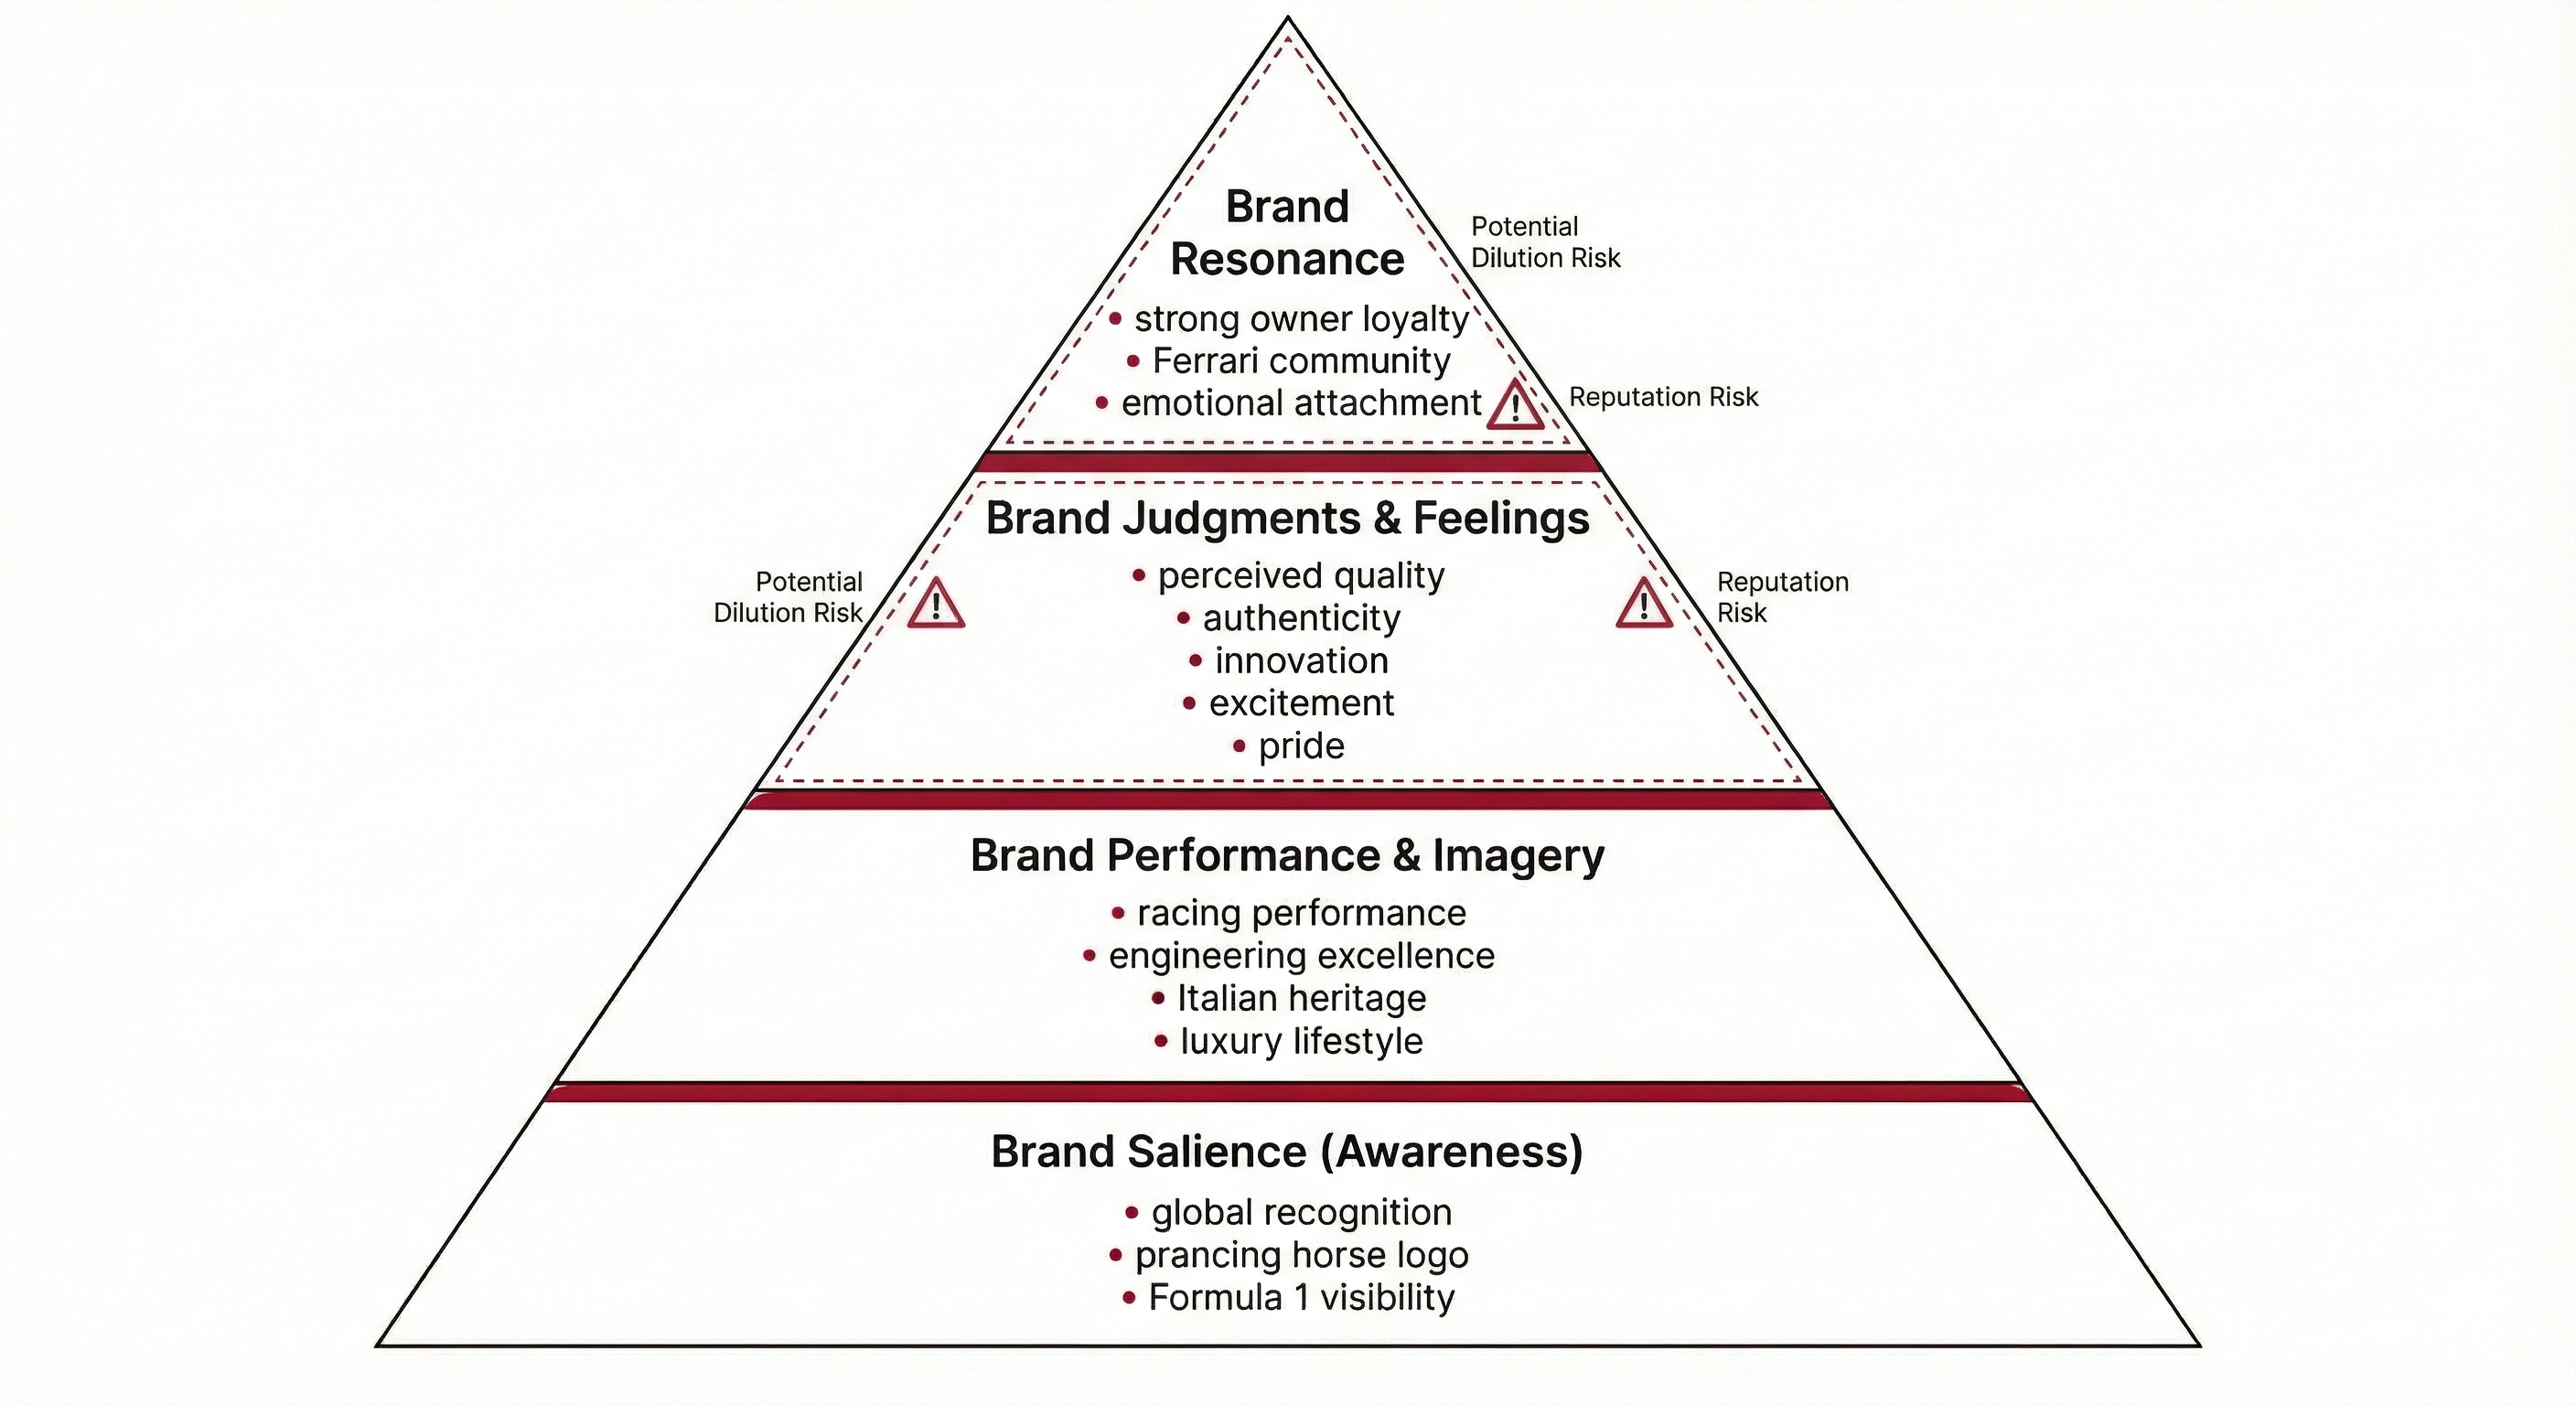
\includegraphics[width=0.8\textwidth]{../team/12.1.png}
%\fbox{\parbox{0.9\textwidth}{\vspace{1.2cm}\centering [Figure 10: Brand Equity Pyramid (Ferrari Placeholder)]\vspace{1.2cm}}}
\caption{Brand equity pyramid.}
\end{figure}

% ============================================================
% Chapter 13
% ============================================================
\chapter{Marketing Mix Deep Dive: Product, Place, and Promotion (Ferrari)}
\section{Product Strategy and Portfolio Architecture}
Ferrari's product strategy can be understood as a portfolio system that balances core models (supporting brand continuity and broader qualified demand) with special series and limited editions (supporting scarcity, collector demand, and cultural impact). Product decisions must protect long-term brand equity by maintaining coherent design language and credible performance improvements.

Important product strategy considerations include:
\begin{itemize}[leftmargin=*]
  \item \textbf{Line extension discipline:} avoid adding variants that create confusion or reduce perceived rarity.
  \item \textbf{Customization governance:} enable personalization while preserving recognizable Ferrari identity.
  \item \textbf{Lifecycle planning:} manage introductions and updates to maintain anticipation and reduce demand volatility.
  \item \textbf{Quality and reliability signaling:} ensure the ownership experience reinforces premium positioning.
\end{itemize}

\section{Place: Selective Distribution and Retail Experience}
In luxury, distribution is a strategic control system. Selective distribution ensures that retail environments match brand standards. Ferrari dealerships and brand spaces function as theaters of the brand: physical evidence of craftsmanship, heritage, and exclusivity.

Key place-related themes include:
\begin{itemize}[leftmargin=*]
  \item \textbf{Dealer governance:} standards for service quality, showroom design, and messaging.
  \item \textbf{Geographic coverage:} sufficient presence to serve owners while avoiding overexposure.
  \item \textbf{Experience design:} delivery ceremonies, curated events, and ownership rituals.
\end{itemize}

\section{Promotion: Storytelling, PR, and Experiential Communications}
Ferrari's promotion is best understood as curated storytelling rather than persuasion through price. Racing, heritage content, design narratives, and innovation announcements form an integrated communication system.

An academic evaluation can examine:
\begin{itemize}[leftmargin=*]
  \item \textbf{Message themes:} performance, craftsmanship, heritage, innovation, exclusivity.
  \item \textbf{Channel fit:} where premium storytelling is credible and where it risks overexposure.
  \item \textbf{Experiential strategy:} how events create belonging and reinforce loyalty.
\end{itemize}

\begin{figure}[H]
\centering
\includegraphics[width=0.5\textwidth]{../team/13.1.png}
%\fbox{\parbox{0.9\textwidth}{\vspace{1.2cm}\centering [Figure 11: Ferrari Marketing Mix System Map Placeholder]\vspace{1.2cm}}}
\caption{Marketing mix system map.}
\end{figure}

% ============================================================
% Chapter 14
% ============================================================
\chapter{Application of Economic Principles to Ferrari\textquotesingle s Business Model}
\section{Scarcity, Allocation, and Perceived Value}
In economics, scarcity increases value when demand exceeds supply. Luxury brands often institutionalize scarcity through capacity constraints, limited editions, and controlled distribution. For Ferrari, scarcity can create waiting lists and preserve resale values, reinforcing desirability. However, scarcity must be managed carefully: artificial scarcity without credible craftsmanship can damage trust.

\section{Differentiation and Monopolistic Competition}
Ferrari differentiates through design language, performance engineering, heritage authenticity, and experience ecosystems. Differentiation shifts demand by creating unique perceived benefits and reduces substitutability, supporting higher markups.

\section{Two-Sided Value: Owners and Aspirational Audience}
Ferrari's economic ecosystem includes a large aspirational audience that may never purchase a car but consumes content, merchandise, and brand symbolism. This audience strengthens brand awareness and cultural capital. The firm must manage this two-tier ecosystem so that accessibility (visibility) does not erode exclusivity.

\section{Dynamic Competition and Innovation}
Dynamic competition emphasizes innovation over static price competition. Ferrari invests in new technologies, performance improvements, and design updates to maintain its position. The innovation pipeline influences expectations and hence demand today (anticipation effects).

\section{Externalities and Regulation}
Automotive production and usage impose externalities such as emissions and congestion. Regulation internalizes some externalities through standards and taxes. For Ferrari, the strategic response involves technology transition, product planning, and communications that align performance with compliance and sustainability narratives.

\begin{table}[H]
\centering
\caption{Economic principles applied to Ferrari.}
\begin{tabularx}{0.95\textwidth}{@{}p{0.26\textwidth}X@{}}
  	\toprule
  	\textbf{Dimension} & \textbf{Ferrari evidence and interpretation }\\
\midrule
Scarcity & Smaintains intentionally limited production volumes relative to global demand. This engineered scarcity enhances perceived exclusivity and supports a strategy to protect its brand integrity. \\
Differentiation & Ferrari's differentiation stems from a combination of performance engineering, distinctive design language, racing heritage, and a curated ownership experience. Strong differentiation reduces price elasticity and shifts competition away from cost-based factors toward symbolic value and emotional appeal.\\
Durable goods & Ferrari vehicles are long-lasting luxury durable goods with high residual values. Certified pre-owned programs, scheduled maintenance, and personalised after-sales services reinforce trust and influence long-term demand. The strong secondary market further reinforces the brand's value proposition.\\
Oligopoly rivalry & operates within a narrow high-performance luxury oligopoly that includes firms such as Lamborghini, McLaren, and Porsche. Competitive dynamics focus on innovation, technology integration, design evolution, and narrative storytelling rather than price competition. \\
Regulation/externalities & DEnvironmental regulations and emissions standards significantly shape Ferrari's technology roadmap. The company has increased investment in hybrid and electrification technologies to comply with European regulations stringently.\\
\bottomrule
\end{tabularx}
\end{table}

% ============================================================
% Chapter 15
% ============================================================
\chapter{SWOT Analysis}
\section{Strengths}
\begin{itemize}[leftmargin=*]
  \item Iconic global brand with strong heritage and authenticity.
  \item High differentiation and premium pricing power.
  \item Strong community and experiential ecosystem.
  \item Engineering excellence and motorsport credibility.
\end{itemize}

\section{Weaknesses}
\begin{itemize}[leftmargin=*]
  \item Reliance on brand reputation; high sensitivity to reputational risks.
  \item Capacity constraints can limit growth and may frustrate demand.
  \item High costs of innovation, compliance, and maintaining craftsmanship.
  \item Complexity from customization and low-volume production.
\end{itemize}

\section{Opportunities}
\begin{itemize}[leftmargin=*]
  \item Digitally enhanced clienteling and personalization.
  \item Sustainable innovation that preserves performance identity.
  \item Emerging markets with growing luxury segments.
  \item Expanded experience offerings and services increasing lifetime value.
\end{itemize}

\section{Threats}
\begin{itemize}[leftmargin=*]
  \item Regulatory tightening (emissions, noise, safety, data).
  \item Macroeconomic downturns affecting discretionary luxury demand.
  \item Competitive moves from luxury rivals and tech-forward entrants.
  \item Brand dilution risks from overexposure or misaligned partnerships.
\end{itemize}

\begin{figure}[H]
\centering
\includegraphics[width=0.8\textwidth]{../team/15.1.png}
%\fbox{\parbox{0.9\textwidth}{\vspace{1.2cm}\centering [Figure 8: SWOT Matrix (Ferrari Placeholder)]\vspace{1.2cm}}}
\caption{SWOT matrix.}
\end{figure}

% ============================================================
% Chapter 16
% ============================================================
\chapter{Challenges, Opportunities, and Future Marketing Strategies}
\section{Strategic Challenges}
\subsection{Balancing Growth and Exclusivity}
Ferrari faces an inherent tension: growth objectives can conflict with scarcity-based brand equity. The strategic challenge is to expand value capture without expanding volume in ways that reduce desirability.

\subsection{Technology Transition Without Identity Loss}
Shifts toward electrification and software-defined vehicles may challenge Ferrari's traditional identity based on sound, mechanical feel, and motorsport heritage. Marketing must frame innovation as consistent with Ferrari's essence rather than as a departure.

\subsection{Reputation and Social Expectations}
Luxury brands are increasingly evaluated on sustainability, labor practices, and transparency. Ferrari must manage corporate narratives credibly to avoid accusations of greenwashing or superficial CSR.

\section{Opportunities for Marketing Strategy}
\subsection{High-Touch Digital Clienteling}
Ferrari can expand relationship marketing by integrating CRM data with bespoke experiences: personalized content, invitations, and service communications.

\subsection{Experience-Led Brand Extensions}
Experience products (track events, factory tours, curated travel) can deepen loyalty and create additional revenue streams with lower dilution risk than mass merchandise.

\subsection{Community Governance and Advocacy}
Owner clubs and enthusiast communities can act as advocacy networks. Strategic community governance (standards, events, co-creation) can protect brand meaning.

\section{Future Strategy Proposals (Structured Recommendations)}
The following proposals are presented as structured strategic initiatives.

\subsection{Strategy 1: Scarcity-Consistent Product Portfolio Management}
\begin{itemize}[leftmargin=*]
  \item Maintain clear separation between core models and limited series.
  \item Use allocation mechanisms and client history to reward loyalty.
  \item Increase customization depth rather than production volume to grow value.
\end{itemize}

\subsection{Strategy 2: Digital-First Relationship Marketing}
\begin{itemize}[leftmargin=*]
  \item Strengthen account-based personalization while respecting privacy.
  \item Integrate website touchpoints with dealership CRM for consistent journeys.
  \item Use content to educate and build anticipation (innovation storytelling).
\end{itemize}

\subsection{Strategy 3: Sustainability as Engineering Excellence}
\begin{itemize}[leftmargin=*]
  \item Frame sustainability as performance engineering and responsible innovation.
  \item Provide transparent reporting and measurable initiatives (placeholders in Appendix).
  \item Ensure marketing claims are evidence-based to protect credibility.
\end{itemize}

\begin{table}[H]
\centering
\caption{Strategic initiatives roadmap.}
\begin{tabularx}{0.95\textwidth}{@{}p{0.22\textwidth}p{0.18\textwidth}X@{}}
\toprule
\textbf{Initiative} & \textbf{Time horizon} & \textbf{Key actions and success metrics (placeholder)}\\
\midrule
Digital clienteling & 6--18 months & \begin{itemize}
                    \item CRM integration
                    \item Personalization
                    \item Privacy controls
                \end{itemize}\\
Experience expansion & 12--24 months & \begin{itemize}
                    \item Curated events
                    \item Owner journeys
                    \item Conversion to repeat purchase
                \end{itemize}\\
Sustainability narrative & 12--36 months & \begin{itemize}
                    \item Transparent reporting
                    \item Technology milestones
                    \item Reputation indicators
                \end{itemize}\\
\bottomrule
\end{tabularx}
\end{table}

% ============================================================
% Chapter 17 (sharaf)
% ============================================================
\chapter{Implementation, Control, and Metrics}

\section{Why Control Systems Matter in Luxury}
Marketing strategy is only as effective as its implementation. In luxury contexts, implementation failures can be especially costly because they generate reputational damage rather than merely lost sales. Therefore, Ferrari requires control systems that monitor service quality, communication coherence, and customer experience consistency.

In academic terms, control systems provide feedback loops that reduce variance in service delivery and protect the brand promise. They also reduce internal principal--agent problems, where local commercial incentives could otherwise encourage decisions that conflict with long-term brand stewardship.

% -----------------------------------------------------------
% SECTION 17.2: BALANCED SCORECARD
% -----------------------------------------------------------
\section{Balanced Scorecard for Ferrari Marketing}
A balanced scorecard approach can translate strategy into measurable objectives across four perspectives: financial, customer, internal process, and learning/innovation.

% [H] forces the table to stay RIGHT HERE.
\begin{table}[H] 
    \small
    \centering
    \renewcommand{\arraystretch}{1.2} % Slightly tighter to save space
    \caption{Balanced Scorecard for Ferrari Marketing Control}
    \label{tab:balanced_scorecard}
    
    \begin{tabularx}{\textwidth}{@{} >{\bfseries}l >{\raggedright\arraybackslash}X >{\raggedright\arraybackslash}X @{}}
        \toprule
        Perspective & \textbf{Objectives} & \textbf{Measures / Targets} \\ 
        \midrule
        
        Financial & 
        Protect premium margins; grow value of services. & 
        Maintain/increase EBIT margin; 15\% growth in revenue from ``Tailor Made'' and Bespoke services [4, 5]. \\ 
        \addlinespace
        
        Customer & 
        Increase brand loyalty and community advocacy. & 
        $>$80\% repeat purchase rate; NPS above 70; 20\% growth in official club memberships [4, 5]. \\ 
        \addlinespace
        
        Internal Process & 
        Improve customer journey consistency and digital integration. & 
        $<$24-hour response time for dealer leads; 100\% compliance with global retail experience standards [4, 5]. \\ 
        \addlinespace
        
        Learning/Innov. & 
        Strengthen digital capabilities and sustainability. & 
        Completion of digital clienteling training; achievement of key hybrid/EV technology milestones [4, 5]. \\ 
        \bottomrule
    \end{tabularx}
\end{table}

% -----------------------------------------------------------
% SECTION 17.3: RISK REGISTER
% -----------------------------------------------------------
% This will now appear immediately AFTER the table above.
\section{Risk Register}
The following risk register outlines potential strategic threats and the mitigation strategies required to protect brand equity.

% [H] forces this table to stay RIGHT HERE too.
\begin{table}[H]
    \centering
    \small
    \renewcommand{\arraystretch}{1.2}
    \caption{Marketing and Strategic Risk Register}
    \label{tab:risk_register}
    
    \begin{tabularx}{\textwidth}{@{} >{\bfseries}l c c >{\raggedright\arraybackslash}X @{}}
        \toprule
        Risk Event & \textbf{Prob.} & \textbf{Imp.} & \textbf{Mitigation Strategy} \\ 
        \midrule
        
        Brand Dilution & 
        Med & High & 
        Strict scarcity discipline; rigorous partnership governance; consistent global retail standards [7]. \\ 
        \addlinespace
        
        Cyber/Privacy & 
        Low & High & 
        ``Privacy-by-Design''; security audits of CRM/owner portals; incident response protocols [7]. \\ 
        \addlinespace
        
        Regulatory Shift & 
        High & High & 
        Accelerated R\&D in electrification; tech roadmapping; framing sustainability as ``engineering excellence'' [7]. \\ 
        \addlinespace
        
        Macro Downturn & 
        Med & Med & 
        Geographic diversification; strengthening counter-cyclical revenue (aftersales/experiences) [7]. \\ 
        \bottomrule
    \end{tabularx}
\end{table}

% ============================================================
% Chapter 18
% ============================================================
\chapter{Conclusion and Recommendations}
\section{Conclusion}
This report applied core economics and marketing concepts to Ferrari to explain how the firm creates value through differentiation, scarcity management, and relationship-based brand stewardship. Economic principles clarify how premium pricing and limited supply can sustain pricing power and protect long-run profitability, while marketing frameworks explain how Ferrari maintains desirability through storytelling, controlled distribution, experiential touchpoints, and community management. The analysis shows that Ferrari's competitive advantage is not reducible to engineering alone; rather, it is the integration of engineering excellence with coherent brand meaning and carefully designed customer experiences.

\section{Recommendations}
\begin{enumerate}[label=\textbf{R\arabic*:},leftmargin=*]
  \item Preserve scarcity and exclusivity by prioritizing value growth through customization, services, and experiences rather than volume.
  \item Strengthen digital relationship marketing (clienteling) via CRM integration, personalization, and privacy-first trust-building.
  \item Align technology transition communications with Ferrari's identity by framing sustainability and innovation as expressions of performance excellence.
  \item Expand measurable marketing control systems: define KPIs across brand equity, community engagement, lead quality, and owner retention.
  \item Build risk governance around reputation: partnership screening, messaging consistency, and crisis response protocols.
\end{enumerate}

% ============================================================
% References
% ============================================================
\cleardoublepage
\printbibliography

% ============================================================
% Appendices (adds depth and page count)
% ============================================================
\appendix
\chapter{Appendix A: Expanded Marketing Mix (7Ps) for Ferrari (Template)}
\section{Product}
Discuss core product layers: core benefit (performance/identity), actual product (vehicle design, specs), augmented product (services, warranty, events). Insert model-by-model comparative table.

\section{Price}
Discuss premium pricing, line pricing, psychological pricing in luxury, and allocation mechanisms. Include placeholders for elasticity analysis.

\section{Place (Distribution)}
Discuss selective distribution, dealership experience standards, geographic strategy, and channel governance.

\section{Promotion}
Discuss IMC, brand storytelling, PR strategy, experiential marketing, partnerships.

\section{People}
Discuss client advisors, dealership staff training, event hosts, and service technicians.

\section{Process}
Discuss customer journey processes: inquiry to allocation, purchase, delivery ceremony, aftersales.

\section{Physical Evidence}
Discuss showrooms, packaging, documentation, delivery experience, digital interfaces.

\begin{table}[H]
\centering
\caption{7Ps worksheet.}
\begin{tabularx}{0.95\textwidth}{@{}p{0.12\textwidth}X X@{}}
\toprule
\textbf{P} & \textbf{Description } & \textbf{Ferrari-specific notes  }\\
\midrule
Product & Multi-layered product including core benefits (performance, prestige, brand identity), actual product (high-performance sports cars). & Ferrari offers limited production models, special series (Icona, Speciale), and extensive personalization through Ferrari Atelier.\\
Price & Premium pricing strategy based on scarcity, craftsmanship, and brand equity rather than cost-based pricing. & High prices signal luxury and exclusivity. Limited availability and strong resale value justify premium pricing.\\
Place & Selective and tightly controlled global distribution through authorized dealerships. & Ferrari limits dealership numbers to maintain exclusivity and brand control, ensuring consistent luxury standards.\\
Promotion & Integrated marketing communications focused on heritage, racing success, innovation, and brand storytelling. & Formula 1 participation acts as a global promotional platform. Ferrari relies more on PR and events than mass advertising.\\
People & Highly trained sales consultants, brand specialists, and service staff delivering personalized customer interactions. & Employees act as brand ambassadors, offering high-touch service aligned with Ferrari’s luxury positioning.\\
Process & Customized and relationship-driven purchasing process, from allocation and configuration to delivery. & Long waiting lists, invitation-only purchases for special models, and exclusive owner events enhance loyalty.\\
Physical Evidence & Tangible cues that reflect luxury and heritage, including showrooms, packaging, and digital interfaces. & Ferrari showrooms resemble luxury galleries, supported by museums and racing artifacts that reinforce authenticity.\\
\bottomrule
\end{tabularx}
\end{table}

%(sharaf)
\chapter{Appendix B: Customer Journey Map and Touchpoints}

\section{Strategic Stages and Touchpoints}

Table B.1 below details the six stages of the Ferrari customer journey, mapping specific touchpoints to customer goals and strategic metrics.

% -----------------------------------------------------------
% TABLE B.1: LONGTABLE VERSION (Flows across pages)
% -----------------------------------------------------------
% Column widths: 12% | 27% | 27% | 27% (Sums to ~93% to fit margins)
\begin{longtable}{@{} p{0.12\textwidth} p{0.27\textwidth} p{0.27\textwidth} p{0.27\textwidth} @{}}
    
    \caption{Detailed Customer Journey Map and Strategic Touchpoints for Ferrari} \\
    \toprule
    \textbf{Stage} & \textbf{Customer Goals} & \textbf{Key Touchpoints} & \textbf{Metrics \& Risks} \\ 
    \midrule
    \endfirsthead

    % This header appears on the NEXT page
    \multicolumn{4}{c}{{\bfseries \tablename\ \thetable{} -- continued from previous page}} \\
    \toprule
    \textbf{Stage} & \textbf{Customer Goals} & \textbf{Key Touchpoints} & \textbf{Metrics \& Risks} \\ 
    \midrule
    \endhead

    \bottomrule
    \multicolumn{4}{r}{{Continued on next page...}} \\ 
    \endfoot

    \bottomrule
    \endlastfoot

    % --- ROW 1: AWARENESS ---
    \textbf{Awareness} & 
    Discover brand meaning, racing heritage, and identity signaling. & 
    \begin{itemize}[leftmargin=*, nosep]
        \item F1 Racing and Motorsport achievements.
        \item Official Website (Storytelling/Heritage).
        \item Global PR (Design awards/Product reveals).
        \item Social Media (Racing/Lifestyle content).
    \end{itemize} & 
    \textbf{Metrics:} Global reach, brand sentiment, cultural visibility. \par
    \vspace{0.3em}
    \textbf{Risks:} Brand dilution through overexposure; loss of racing credibility. \\ 
    \addlinespace[1.5em] % Adds breathing room between rows
    
    % --- ROW 2: CONSIDERATION ---
    \textbf{Consideration} & 
    Evaluate model fit, performance specs, and access levels. & 
    \begin{itemize}[leftmargin=*, nosep]
        \item Online Digital Configurator and Model Pages.
        \item Initial Dealer Contact and Showroom Visits.
        \item Exclusive Private Events and Factory content.
        \item Personalised Account/Digital Services.
    \end{itemize} & 
    \textbf{Metrics:} Qualified lead rate, engagement depth, lead response time. \par
    \vspace{0.3em}
    \textbf{Risks:} Inconsistent dealer response; website UX friction. \\ 
    \addlinespace[1.5em]

    % --- ROW 3: ACQUISITION ---
    \textbf{Acquisition} & 
    Secure vehicle allocation and finalize bespoke contracts. & 
    \begin{itemize}[leftmargin=*, nosep]
        \item One-on-one Client Advisor consultations.
        \item ``Tailor Made'' or Atelier Bespoke sessions.
        \item Financing, Warranty, and Service Contracts.
        \item Allocation status and Waitlist management.
    \end{itemize} & 
    \textbf{Metrics:} Conversion rate (lead to deposit); revenue from customization. \par
    \vspace{0.3em}
    \textbf{Risks:} Perceived unfairness in allocation; compliance/legal errors. \\ 
    \addlinespace[1.5em]
    
    % --- ROW 4: DELIVERY ---
    \textbf{Delivery} & 
    Celebrate ownership entry and join the exclusive community. & 
    \begin{itemize}[leftmargin=*, nosep]
        \item Factory Delivery Ceremony (Maranello).
        \item Local Showroom Handover and Onboarding.
        \item Ownership Rituals (Artifacts/packaging).
        \item Official Factory Tours and Museum access.
    \end{itemize} & 
    \textbf{Metrics:} Initial satisfaction score; Advocacy intent. \par
    \vspace{0.3em}
    \textbf{Risks:} Physical evidence mismatch (showroom quality); poor ceremony execution. \\ 
    \addlinespace[1.5em]

    % --- ROW 5: OWNERSHIP ---
    \textbf{Ownership} & 
    Maintain performance and deepen the relationship via experiences. & 
    \begin{itemize}[leftmargin=*, nosep]
        \item Certified Pre-owned and Aftersales.
        \item Official Owner Clubs and Track Days.
        \item Digital Support Portals and CRM personalization.
        \item Curated Travel and Lifestyle events.
    \end{itemize} & 
    \textbf{Metrics:} Retention rate; service cycle time; digital adoption rate. \par
    \vspace{0.3em}
    \textbf{Risks:} Cyber/Privacy incident (CRM data); service quality variance. \\ 
    \addlinespace[1.5em]
    
    % --- ROW 6: REPURCHASE ---
    \textbf{Repurchase} & 
    Upgrade collection and secure limited series access. & 
    \begin{itemize}[leftmargin=*, nosep]
        \item Exclusive Invitations to Limited Series.
        \item Loyalty-based allocation programs.
        \item Relationship-marketing driven by CRM data.
        \item High-touch invitations to special events.
    \end{itemize} & 
    \textbf{Metrics:} Repeat purchase rate; Customer Lifetime Value (CLV). \par
    \vspace{0.3em}
    \textbf{Risks:} Frustrated demand (waiting lists); loss of loyalty due to poor stewardship. \\ 
    
\end{longtable}

\clearpage

% -----------------------------------------------------------
% FIGURE B.1: CUSTOMER JOURNEY DIAGRAM
% -----------------------------------------------------------
\section{Strategic Ecosystem Map}

Figure B.1 illustrates the integrated flow of the customer journey, highlighting the ``Loyalty Allocation Mechanism'' that routes high-value clients from the Repurchase stage back to priority Acquisition status.

\begin{figure}[htbp]
    \centering
    \resizebox{\textwidth}{!}{%
    \begin{tikzpicture}[
        node distance=1.5cm and 1.2cm,
        stage/.style={
            rectangle, 
            draw=red!80!black, 
            ultra thick, 
            fill=white, 
            text width=6.2cm,
            minimum height=5.2cm, 
            align=left,
            font=\small, 
            drop shadow={opacity=0.2, shadow xshift=3pt, shadow yshift=-3pt},
            rounded corners=4pt,
            inner sep=10pt
        },
        arrow/.style={-{Stealth[scale=1.5]}, red!80!black, ultra thick, rounded corners=5pt}
    ]

    % --- NODES ---
    \node (aware) [stage] {
        \textbf{\large 1. AWARENESS}\\[5pt]
        \rule{6.2cm}{0.5pt} \\[5pt]
        $\bullet$ \textbf{Driver:} Symbolic Utility \& Racing Heritage\\
        $\bullet$ \textbf{Touchpoints:} F1 Scuderia, Global PR, Brand Mythology\\
        $\bullet$ \textbf{Metric:} Cultural Visibility \& Awareness\\[10pt]
        \textit{\scriptsize Ref: Ch 2.1.1, 7.2}
    };

    \node (consid) [stage, right=of aware] {
        \textbf{\large 2. CONSIDERATION}\\[5pt]
        \rule{6.2cm}{0.5pt} \\[5pt]
        $\bullet$ \textbf{Driver:} Digital Storytelling \& Info Asymmetry\\
        $\bullet$ \textbf{Touchpoints:} 3D Configurator, Website, Landing Pages\\
        $\bullet$ \textbf{Metric:} Engagement Depth \& Lead Quality\\[10pt]
        \textit{\scriptsize Ref: Ch 5.2, 12.2}
    };

    \node (acq) [stage, right=of consid] {
        \textbf{\large 3. ACQUISITION}\\[5pt]
        \rule{6.2cm}{0.5pt} \\[5pt]
        $\bullet$ \textbf{Driver:} Scarcity \& Monopolistic Competition\\
        $\bullet$ \textbf{Touchpoints:} Client Advisor, ``Tailor Made'', Waitlists\\
        $\bullet$ \textbf{Metric:} Margin Protection \& Customisation Rev.\\[10pt]
        \textit{\scriptsize Ref: Ch 9.2, 14.1}
    };

    \node (deliv) [stage, below=of acq] {
        \textbf{\large 4. DELIVERY}\\[5pt]
        \rule{6.2cm}{0.5pt} \\[5pt]
        $\bullet$ \textbf{Driver:} Physical Evidence \& Process Quality\\
        $\bullet$ \textbf{Touchpoints:} Factory Ceremony, Handover Rituals\\
        $\bullet$ \textbf{Metric:} Satisfaction Score \& Advocacy Intent\\[10pt]
        \textit{\scriptsize Ref: Appx A.7, 13.2}
    };

    \node (own) [stage, left=of deliv] {
        \textbf{\large 5. OWNERSHIP}\\[5pt]
        \rule{6.2cm}{0.5pt} \\[5pt]
        $\bullet$ \textbf{Driver:} Relationship Marketing (Exp. Economy)\\
        $\bullet$ \textbf{Touchpoints:} Corse Clienti, Owner Clubs, Classiche\\
        $\bullet$ \textbf{Metric:} Service Cycle \& Community Engagement\\[10pt]
        \textit{\scriptsize Ref: Ch 11.4.4, 16.2}
    };

    \node (repur) [stage, left=of own] {
        \textbf{\large 6. REPURCHASE}\\[5pt]
        \rule{6.2cm}{0.5pt} \\[5pt]
        $\bullet$ \textbf{Driver:} Brand Equity \& CLV\\
        $\bullet$ \textbf{Touchpoints:} Icona/Limited Series Invites, Allocation\\
        $\bullet$ \textbf{Metric:} Repeat Purchase \& Resale Value\\[10pt]
        \textit{\scriptsize Ref: Ch 12.3, Rec R1}
    };

    % --- ARROWS ---
    \draw [arrow] (aware) -- (consid);
    \draw [arrow] (consid) -- (acq);
    \draw [arrow] (acq) -- (deliv);
    \draw [arrow] (deliv) -- (own);
    \draw [arrow] (own) -- (repur);

    % --- LOOP ---
    \draw [arrow, dashed] (repur.west) 
        -- ++(-1.0, 0)                  
        |- ($(acq.north) + (0, 1.8)$)   
        -| (acq.north);                 

    % --- LABEL ---
    \node [fill=white, draw=red!80!black, font=\bfseries\scriptsize, rounded corners] 
        at ($(consid.north) + (0, 1.8)$) {LOYALTY ALLOCATION MECHANISM};

    \end{tikzpicture}
    }
    \caption{The Ferrari Customer Journey: Integrated Strategic Touchpoints and Economic Value Cycle.}
    \label{fig:customer_journey_final}
\end{figure}

\chapter{Appendix C: Microeconomic Model}
\section{Elasticity Estimation}

In the absence of transaction-level market data, an illustrative elasticity estimation is performed using synthetically generated observations. This appendix demonstrates the estimation methodology without making empirical claims.

The log--log demand model is specified as:

\begin{equation}
\ln(Q) = \alpha + \beta \ln(P) + \gamma X + \varepsilon
\end{equation}

where $Q$ denotes quantity demanded, $P$ represents price, $X$ is a control variable, and $\varepsilon$ is a stochastic error term. The coefficient $\beta$ represents the price elasticity of demand.

\subsection*{MATLAB Implementation}

\begin{lstlisting}[caption={Log--log elasticity estimation using illustrative data}]
clc; clear; close all;

% Reproducibility
rng(1);

% Number of observations
n = 100;

% Synthetic price data
P = exp(2 + 0.3 * randn(n,1));

% Control variable (income proxy)
X = 50 + 10 * randn(n,1);

% Assumed true elasticity
beta_true = -0.8;

% Generate quantity demanded
Q = exp(5 + beta_true * log(P) + 0.02 * X + 0.2 * randn(n,1));

% Log transformations
lnQ = log(Q);
lnP = log(P);

% Regression matrix
Z = [ones(n,1), lnP, X];

% Ordinary Least Squares
b = (Z' * Z) \ (Z' * lnQ);

% Extract elasticity
beta_hat = b(2);

fprintf('Estimated price elasticity:\n');
fprintf('   %.4f\n', beta_hat);
\end{lstlisting}

\subsection*{Estimation Result}

The illustrative estimation yields the following price elasticity:

\begin{equation}
\hat{\beta} = -0.796
\end{equation}

This value indicates moderately inelastic demand, where quantity demanded responds proportionally less than price changes, consistent with standard economic theory.

---

\section{Cost Structure Discussion}

The cost structure is decomposed into fixed and variable components. Fixed costs include research and development, tooling, compliance, branding, and administrative overheads, which are independent of production volume in the short run.

Variable costs scale with output and include materials, labor, energy consumption, and logistics. The assumed cost proportions are used for illustrative purposes only.

\subsection*{MATLAB Cost Structure Visualization}

\begin{lstlisting}[caption={Illustrative cost structure visualization}]
% Cost structure percentages
fixed_costs    = 45;
variable_costs = 55;

costs = [fixed_costs, variable_costs];
labels = {'Fixed Costs', 'Variable Costs'};

figure;
pie(costs, labels);
title('Illustrative Cost Structure Breakdown');
colormap([0.25 0.2 0.7; 1 1 0]);
\end{lstlisting}

\begin{figure}[h]
\centering
\includegraphics[width=0.6\textwidth]{../team/c1.png}
\caption{Illustrative cost structure breakdown.}
\label{fig:cost_structure}
\end{figure}

\chapter{Appendix D: Competitive Set and Positioning Map (Template)}
\section{Competitive Set Definition}
Define the competitive set by price tier, performance benchmarks, heritage, and exclusivity. Include direct luxury performance rivals and adjacent lifestyle competitors.

\section{Perceptual Mapping}
Construct a 2D positioning map, for example:
\begin{itemize}[leftmargin=*]
  \item Axis 1: ``Heritage authenticity'' (low to high)
  \item Axis 2: ``Performance/technology intensity'' (low to high)
\end{itemize}

\begin{figure}[H]
\centering
\includegraphics[width=0.8\textwidth]{../team/d1.png}
%\fbox{\parbox{0.9\textwidth}{\vspace{1.2cm}\centering [Figure A3: Perceptual Map Placeholder (Ferrari vs. Rivals)]\vspace{1.2cm}}}
\caption{Perceptual map placeholder.}
\end{figure}

\chapter{Appendix E: Data Collection Plan (For Academic Rigor)}
\section{Primary Data (Optional)}
\begin{itemize}[leftmargin=*]
  \item Structured interviews with owners/dealership staff (subject to ethics approval).
  \item Survey on brand perceptions and motivations (collectors vs. drivers).
\end{itemize}

\section{Secondary Data}
\begin{itemize}[leftmargin=*]
  \item Official corporate publications and investor relations materials.
  \item Public web analytics proxies and social engagement indicators.
  \item Industry reports on luxury goods and automotive trends.
\end{itemize}

\section{Ethics and Confidentiality}
Ensure informed consent, anonymity, and careful treatment of personal data, consistent with academic policy and data protection law.

\chapter{Appendix F: TOWS Matrix (From SWOT to Strategy)}
The TOWS matrix translates SWOT observations into actionable strategies. This appendix is intentionally structured as a write-in template so that the report can be strengthened with evidence-based strategy statements and expanded into short paragraphs for submission.

\begin{table}[H]
\centering
\caption{TOWS matrix template to translate SWOT into actions.}
\begin{tabularx}{1\textwidth}{@{}p{0.14\textwidth}X X@{}}
  \toprule
 & \textbf{Opportunities (O)} & \textbf{Threats (T)}\\
\midrule
  \textbf{Strengths (S)} & 
                \textbf{SO Strategies (Strengths–Opportunities)} \newline 
                Ferrari can effectively leverage its unparalleled brand reputation and racing-derived technological capabilities to capitalise on the transition toward hybrid and electric luxury mobility. The company’s proven ability to transfer innovations from Formula 1 to its road-going fleet allows it to meet stringent sustainability expectations while enhancing performance. \newline
                Additionally, Ferrari can exploit the rising demand in emerging luxury markets by offering highly exclusive, limited-edition models and bespoke personalisation options. This ensures geographical expansion and revenue growth without compromising the brand’s core strategy of engineered scarcity. & 
                \textbf{ST Strategies (Strengths–Threats)} \newline 
                Ferrari’s exceptional brand loyalty and substantial pricing power serve as a buffer against external threats like shifting environmental regulations and intensified competition. By maintaining its lead in powertrain efficiency and alternative energy research, the firm remains a proactive pioneer rather than a reactive follower in the face of legal mandates. \newline
                Simultaneously, the brand’s focus on artisanal craftsmanship and heritage protects it from price wars. Unlike mass-market luxury manufacturers, Ferrari’s low-volume model reduces financial exposure to global economic downturns and aggressive rival positioning. \tabularnewline
                \hline
                
                \textbf{Weaknesses (W)} & 
                \textbf{WO Strategies (Weaknesses–Opportunities)} \newline 
                The challenges of high production costs and limited industrial scalability can be mitigated by integrating advanced digital ecosystems and customer data analytics. Enhanced digital engagement can refine demand forecasting and relationship management, leading to leaner production processes and reduced operational overhead. \newline
                Furthermore, Ferrari can address its internal R\&D limitations in specific electrification domains by establishing selective, high-level partnerships with specialist technology firms. This allows for rapid innovation and access to cutting-edge expertise while protecting the firm’s capital and focusing on its core design DNA. & 
                \textbf{WT Strategies (Weaknesses–Threats)} \newline 
                To defend against combined internal vulnerabilities and external market threats, Ferrari must maintain a rigorous and cautious strategic posture. Tight control over licensing and brand extensions is vital to prevent brand dilution and ensure that every collaboration reinforces Ferrari’s premium standing. \newline
                Moreover, strict financial discipline coupled with highly flexible production planning allows the company to navigate economic volatility. By keeping supply intentionally below market demand, Ferrari preserves its long-term brand equity and limits financial risk during periods of global market instability. \tabularnewline
                \hline\\
\bottomrule
\end{tabularx}
\end{table}

\chapter{Appendix G: Figures and Tables Submission Index (Checklist)}
This appendix provides a structured index of placeholders used in this report. It can be used as a submission checklist to ensure that required visual evidence (screenshots, organization charts, positioning maps, etc.) is added later if permitted.

\section{Figure Placeholders}
\begin{longtable}{@{}p{0.16\textwidth}p{0.76\textwidth}@{}}
  \toprule
  \textbf{ID} & \textbf{Placeholder description}\\
\midrule
Figure 1 & Research framework linking economics and marketing to Ferrari\\
Figure 2 & Ferrari business model overview (luxury + performance + experiences)\\
Figure 3 & Ferrari organizational structure (high-level)\\
Figure 4 & Ferrari website UX evidence placeholder\\
Figure 5 & IMC map (paid/owned/earned media)\\
Figure 6 & Pricing architecture ladder\\
Figure 7 & Porter five forces diagram\\
Figure 8 & SWOT matrix\\
Figure 9 & Trend map (electrification, software, sustainability, experience economy)\\
Figure 10 & Brand equity pyramid\\
Figure 11 & Marketing mix system map\\
Figure A1 & Customer journey diagram\\
Figure A2 & Cost structure chart\\
Figure A3 & Perceptual/positioning map\\
\bottomrule
\end{longtable}

\section{Table Placeholders}
\begin{longtable}{@{}p{0.16\textwidth}p{0.76\textwidth}@{}}
  \toprule
  \textbf{ID} & \textbf{Placeholder description}\\
\midrule
Table 1 & Mapping of concepts to Ferrari analysis\\
Table 2 & Decision-rights matrix for luxury governance\\
Table 3 & Website audit checklist\\
Table 4 & Ferrari offering portfolio classification\\
Table 5 & Digital KPIs template\\
Table 6 & STP summary matrix\\
Table 7 & PESTEL template\\
Table 8 & Economic principles summary\\
Table 9 & Strategic initiatives roadmap\\
Table 10 & Brand equity diagnostic template\\
Table 11 & Balanced scorecard template\\
Table 12 & Risk register template\\
Table A1 & 7Ps worksheet\\
Table B1 & Customer journey touchpoints table\\
Table F1 & TOWS matrix template\\
\bottomrule
\end{longtable}

\end{document}
